% Chapter 10: State space models, Kalman filter and Markov switching
% Time Series Analysis -- Bachelor's programmes Economic Informatics and Economic Cybernetics, Bucharest University of Economic Studies
% GENERATED by latex/build_chapter10.py -- edit the generator, not this file.

\newcommand{\coursename}{Time Series Analysis}
% Preambul comun TSA -- Serii de timp / Time Series Analysis (Beamer, 16:9)
% Același design ca MFM și SFM (preluat din SFM, 5 octombrie 2026). Înainte de % Preambul comun TSA -- Serii de timp / Time Series Analysis (Beamer, 16:9)
% Același design ca MFM și SFM (preluat din SFM, 5 octombrie 2026). Înainte de % Preambul comun TSA -- Serii de timp / Time Series Analysis (Beamer, 16:9)
% Același design ca MFM și SFM (preluat din SFM, 5 octombrie 2026). Înainte de \input{../../latex/preamble} se definește
%   \newcommand{\coursename}{Time Series Analysis}      (EN)
%   \newcommand{\coursename}{Serii de timp}       (RO)  și  \def\tsalang{ro}
% Fișierele .tex se află în EN/Courses, EN/Seminars, RO/Cursuri, RO/Seminarii (două niveluri sub rădăcină).
% Deck-urile sînt generate de latex/build_chapterN.py / build_seminarN.py (vezi latex/tsa_build.py).

\documentclass[9pt, aspectratio=169, t]{beamer}
\providecommand{\coursename}{Time Series Analysis}

% Ensure content fits on slides
\setbeamersize{text margin left=8mm, text margin right=8mm}
% Smaller institute font (title page)
\setbeamerfont{institute}{size=\footnotesize}

%=============================================================================
% THEME AND STYLE CONFIGURATION
%=============================================================================
\usetheme{default}
% Using default theme for clean header/footer control

% Color Palette (matching Redispatch PDF)
\definecolor{MainBlue}{RGB}{26, 58, 110}
\definecolor{AccentBlue}{RGB}{26, 58, 110}
\definecolor{IDAred}{RGB}{205, 0, 0}
\definecolor{DarkGray}{RGB}{51, 51, 51}
\definecolor{MediumGray}{RGB}{128, 128, 128}
\definecolor{LightGray}{RGB}{248, 248, 248}
\definecolor{VeryLightGray}{RGB}{235, 235, 235}
\definecolor{KeynoteGray}{RGB}{218, 218, 218}
\definecolor{SectionGray}{RGB}{120, 120, 120}
\definecolor{FooterGray}{RGB}{100, 100, 100}
\definecolor{Crimson}{RGB}{220, 53, 69}
\definecolor{Forest}{RGB}{46, 125, 50}
\definecolor{Amber}{RGB}{181, 133, 63}
\definecolor{Orange}{RGB}{230, 126, 34}
\definecolor{Purple}{RGB}{142, 68, 173}

% Gradient background (exact Keynote 315° gradient: white to RGB 218,218,218)
\setbeamertemplate{background}{%
    \begin{tikzpicture}[remember picture, overlay]
        \shade[shading=axis, shading angle=315,
        top color=white, bottom color=KeynoteGray]
        (current page.south west) rectangle (current page.north east);
    \end{tikzpicture}%
}
% Fallback solid color for compatibility
\setbeamercolor{background canvas}{bg=}

\setbeamercolor{palette primary}{bg=MainBlue, fg=white}
\setbeamercolor{palette secondary}{bg=MainBlue!85, fg=white}
\setbeamercolor{palette tertiary}{bg=MainBlue!70, fg=white}
\setbeamercolor{structure}{fg=MainBlue}
\setbeamercolor{title}{fg=IDAred}
\setbeamercolor{frametitle}{fg=IDAred, bg=}
\setbeamercolor{block title}{bg=MainBlue, fg=white}
\setbeamercolor{block body}{bg=VeryLightGray, fg=DarkGray}
\setbeamercolor{block title alerted}{bg=Crimson, fg=white}
\setbeamercolor{block body alerted}{bg=Crimson!8, fg=DarkGray}
\setbeamercolor{block title example}{bg=Forest, fg=white}
\setbeamercolor{block body example}{bg=Forest!8, fg=DarkGray}
\setbeamercolor{item}{fg=MainBlue}

% Footer colors (override Madrid theme blue)
\setbeamercolor{author in head/foot}{fg=FooterGray, bg=}
\setbeamercolor{title in head/foot}{fg=FooterGray, bg=}
\setbeamercolor{date in head/foot}{fg=FooterGray, bg=}
\setbeamercolor{section in head/foot}{fg=FooterGray, bg=}
\setbeamercolor{subsection in head/foot}{fg=FooterGray, bg=}

% Bullet styles (apply everywhere including blocks)
\setbeamertemplate{itemize item}{\color{MainBlue}$\boxdot$}
\setbeamertemplate{itemize subitem}{\color{MainBlue}$\blacktriangleright$}
\setbeamertemplate{itemize subsubitem}{\color{MainBlue}\tiny$\bullet$}
\setbeamertemplate{itemize/enumerate body begin}{\normalsize}
\setbeamertemplate{itemize/enumerate subbody begin}{\normalsize}

% Item spacing - compact style
\setlength{\leftmargini}{10pt}       % Level 1: minimal indent
\setlength{\leftmarginii}{10pt}      % Level 2: minimal additional indent
% Compact list spacing (zero extra space before/after lists in blocks)
\makeatletter
\def\@listi{\leftmargin\leftmargini \topsep 0pt \parsep 0pt \itemsep 0pt}
\def\@listii{\leftmargin\leftmarginii \topsep 0pt \parsep 0pt \itemsep 0pt}
\makeatother

\setbeamertemplate{navigation symbols}{}

%=============================================================================
% CUSTOM HEADLINE
%=============================================================================
\setbeamertemplate{headline}{%
    \vskip10pt%
    \hbox to \paperwidth{%
        \hskip0.5cm%
        {\small\color{FooterGray}\renewcommand{\hyperlink}[2]{##2}\insertsectionhead}%
        \hfill%
        \textcolor{FooterGray}{\small\insertframenumber}%
        \hskip0.5cm%
    }%
    \vskip4pt%
    {\color{FooterGray}\hrule height 0.4pt}%
}

%=============================================================================
% CUSTOM FOOTER
%=============================================================================
\usepackage{fontawesome5}

\setbeamertemplate{footline}{%
    {\color{FooterGray}\hrule height 0.4pt}%
    \vskip4pt%
    \hbox to \paperwidth{%
        \hskip0.5cm%
        \textcolor{FooterGray}{\small\coursename}%
        \hfill%
        \raisebox{-0.1em}{%
            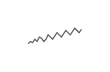
\begin{tikzpicture}[x=0.08em, y=0.08em, line width=0.4pt]
                \draw[FooterGray] (0,3) -- (1,4) -- (2,3.5) -- (3,5) -- (4,4) -- (5,6) -- (6,5.5) -- (7,4) -- (8,5) -- (9,7) -- (10,6) -- (11,5) -- (12,6.5) -- (13,8) -- (14,7) -- (15,6) -- (16,7.5) -- (17,9) -- (18,8) -- (19,7) -- (20,8.5) -- (21,10) -- (22,9) -- (23,8) -- (24,9.5);
            \end{tikzpicture}%
        }%
        \hskip0.5cm%
    }%
    \vskip6pt%
}

%=============================================================================
% PACKAGES
%=============================================================================
\usepackage[utf8]{inputenc}
\DeclareUnicodeCharacter{03B1}{\ensuremath{\alpha}}
\usepackage[T1]{fontenc}
\usepackage{amsmath, amssymb, amsthm}
\usepackage{mathtools}
\usepackage{bm}
\usepackage{tikz}
\usetikzlibrary{arrows.meta, positioning, shapes, calc, decorations.pathreplacing, shadings}
\usepackage{booktabs}
\usepackage{multirow}
\usepackage{array}
\usepackage{graphicx}
\usepackage{animate}
\usepackage{hyperref}
\usepackage{colortbl}
\usepackage{listings}
\lstset{language=Python, basicstyle=\ttfamily\scriptsize, keywordstyle=\color{MainBlue}\bfseries,
  commentstyle=\color{Forest}, stringstyle=\color{Crimson}, breaklines=true,
  frame=none, backgroundcolor=\color{VeryLightGray}, xleftmargin=2mm}
\hypersetup{colorlinks=true, linkcolor=MainBlue, urlcolor=MainBlue}
\graphicspath{{../../logos/}{../../charts/}{../../photos/}}
\usepackage{xcolor}
\hfuzz=2pt  % Suppress tiny overfull warnings (<2pt)
\vfuzz=2pt  % Suppress tiny vertical overfull warnings (<2pt)
% \mathrm in the sans-serif family of the slides (beamer resets \mathrm to the serif family at \begin{document};
% this hook runs after beamer's, so WN, Var, RMSE, ... in formulas match the surrounding text)
% Bold vectors and matrices in the same sans-serif family: \mathbf{A} in sans bold (beamer's own \mathbf came out in
% medium weight), and the bold upright Greek capitals of \boldsymbol / \bm (\bSigma, \bPhi, \boldsymbol{\Theta}) in
% cmss bold: bm.sty fixes its "boldoperators" font when it is loaded (serif cmbx), before beamer switches the
% operators to cmss, so it is reset here.
\AtBeginDocument{%
  \SetMathAlphabet{\mathrm}{normal}{\encodingdefault}{\sfdefault}{\mddefault}{n}%
  \SetMathAlphabet{\mathrm}{bold}{\encodingdefault}{\sfdefault}{bx}{n}%
  \SetMathAlphabet{\mathbf}{normal}{\encodingdefault}{\sfdefault}{bx}{n}%
  \SetMathAlphabet{\mathbf}{bold}{\encodingdefault}{\sfdefault}{bx}{n}%
  \SetSymbolFont{boldoperators}{normal}{OT1}{cmss}{bx}{n}%
  \SetSymbolFont{boldoperators}{bold}{OT1}{cmss}{bx}{n}}

%=============================================================================
% QUANTLET COMMANDS
%   \quantlet{<displayed name>}{<url>}       (generic, compatible with the older TSA decks)
%   \tsaquantlet{Ch_05}{TSA_ch5_garch}       -> https://github.com/danpele/Time-Series-Analysis/tree/main/Quantlets/Ch_05/TSA_ch5_garch
%   \qlurl{<folder>} is defined per chapter by the generator (Quantlets/Ch_NN/<folder>)
%=============================================================================
\newcommand{\tsarepo}{https://github.com/danpele/Time-Series-Analysis}
\newcommand{\tsaqlbase}{https://github.com/danpele/Time-Series-Analysis/tree/main/Quantlets}
\newcommand{\quantlet}[2]{%
    \hfill\href{#2}{%
        \raisebox{-0.15em}{
\includegraphics[height=0.7em]{ql_logo.png}}%
        \textcolor{MainBlue}{\tiny\ #1}%
    }%
}
\newcommand{\tsaquantlet}[2]{\quantlet{\detokenize{#2}}{\tsaqlbase/#1/#2}}

%=============================================================================
% NOTEBOOKS (Google Colab)
%   \colaburl{notebooks/EN/chapter5_seminar_notebook.ipynb} -> the Colab link of a file in the TSA repo
%   \nb: the chapter notebook (each seminar deck redefines it with \renewcommand)
%=============================================================================
\newcommand{\colaburl}[1]{https://colab.research.google.com/github/danpele/Time-Series-Analysis/blob/main/#1}
\newcommand{\nb}{https://colab.research.google.com/github/danpele/Time-Series-Analysis/tree/main/notebooks/EN}
\newcommand{\nbname}{notebooks/EN}

%=============================================================================
% SLIDE HELPERS (used by the generators; the same as in MFM)
%=============================================================================
% local font size for list bodies (the preamble forces \normalsize)
\newcommand{\itemsize}[1]{\setbeamertemplate{itemize/enumerate body begin}{#1}\setbeamertemplate{itemize/enumerate subbody begin}{#1}}
\newcommand{\intitle}[1]{{\hypersetup{urlcolor=white}#1}}   % white links inside coloured title bars
\newcommand{\imgcap}[1]{{\scriptsize #1}\\[0.5mm]}          % caption under a photo
\newcommand{\imgcredit}[2]{{\tiny\color{FooterGray}\href{#1}{#2}}}   % image credit: source URL, author/licence
\newcommand{\aiprompt}[1]{{\ttfamily\color{MainBlue}#1}}     % a prompt to an AI assistant

%=============================================================================
% SEMINARS: student version by default; the instructor wrapper *_solutions.tex sets \solutionstrue
%=============================================================================
\makeatletter\@ifundefined{ifsolutions}{\expandafter\newif\csname ifsolutions\endcsname}{}\makeatother
\newcommand{\solonly}[1]{\ifsolutions #1\fi}
\newcommand{\propsub}{\ifsolutions\else\framesubtitle{\ifdefined\tsalang Rezolvarea se discută la seminar\else Solution discussed in class\fi}\fi}

%=============================================================================
% APPENDIX AND CHAPTER LINKS (latex/appendix_links.py writes the calls; it also re-declares these
% macros before \begin{document}, so the decks compile with or without this preamble block)
%=============================================================================
\providecommand{\tsaapplink}[3]{\hypertarget{#2}{}\hyperlink{#1}{\beamergotobutton{#3}}}
\providecommand{\tsaappback}[2]{\begin{tikzpicture}[remember picture,overlay]\node[anchor=south east] at ([xshift=-3mm,yshift=7mm]current page.south east){\hyperlink{#1}{\beamerreturnbutton{#2}}};\end{tikzpicture}}
\providecommand{\tsachlink}[2]{\href{#1}{#2}}
\providecommand{\tsachlinkt}[2]{\href{#1}{\usebeamercolor[fg]{frametitle}#2}}

%=============================================================================
% QUANTINAR COMMAND: link către un curs Quantinar (subiecte avansate)
%=============================================================================
\newcommand{\quantinar}[2]{%
    \href{#2}{%
        \raisebox{-0.15em}{
\includegraphics[height=0.8em]{qr_logo.png}}%
        \textcolor{MainBlue}{\scriptsize\ #1}%
    }%
}

%=============================================================================
% CUSTOM TITLE PAGE
%=============================================================================
\defbeamertemplate*{title page}{hybrid}[1][]
{
    \vspace{0.2cm}
    % Logos row - top header (with clickable links)
    \begin{center}
        \href{https://www.ase.ro}{
\includegraphics[height=1.0cm]{ase_logo.png}}\hspace{0.3cm}%
        \href{https://theida.net}{
\includegraphics[height=1.0cm]{ida_logo.png}}\hspace{0.3cm}%
        \href{https://blockchain-research-center.com}{
\includegraphics[height=1.0cm]{brc_logo.png}}\hspace{0.3cm}%
        \href{https://www.ai4efin.ase.ro}{
\includegraphics[height=1.0cm]{ai4efin_logo.png}}\hspace{0.3cm}%
        \href{https://ipe.ro/new}{
\includegraphics[height=1.0cm]{acad_logo.png}}\hspace{0.3cm}%
        \href{https://www.digital-finance-msca.com}{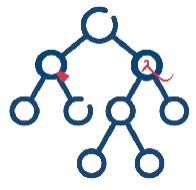
\includegraphics[height=1.0cm]{msca_logo.png}}%
    \end{center}

    \vspace{0.6cm}

    % Main title with Q logos on sides (with clickable links)
    \begin{center}
        \begin{minipage}{0.1\textwidth}
            \centering
            \href{https://quantlet.com}{
\includegraphics[height=1.1cm]{ql_logo.png}}
        \end{minipage}%
        \begin{minipage}{0.78\textwidth}
            \centering
            {\LARGE\bfseries\usebeamercolor[fg]{title}\inserttitle}

            \vspace{0.3cm}

            {\usebeamerfont{subtitle}\usebeamercolor[fg]{title}\insertsubtitle}
        \end{minipage}%
        \begin{minipage}{0.1\textwidth}
            \centering
            \href{https://quantinar.com}{
\includegraphics[height=1.1cm]{qr_logo.png}}
        \end{minipage}
    \end{center}

    \vspace{0.6cm}

    % Authors (left aligned)
    \hspace{0.5cm}{\usebeamerfont{author}\insertauthor}

    \vspace{0.3cm}

    % Institute/Affiliations (left aligned)
    \hspace{0.5cm}\begin{minipage}[t]{0.9\textwidth}
        \raggedright\small\insertinstitute
    \end{minipage}
}

%=============================================================================
% THEOREM ENVIRONMENTS
%=============================================================================
\theoremstyle{definition}
\setbeamertemplate{theorems}[numbered]
\ifdefined\tsalang
\newtheorem{defn}{Definiție}
\newtheorem{thm}{Teoremă}
\newtheorem{prop}{Propoziție}
\newtheorem{rmk}{Observație}
\else
\newtheorem{defn}{Definition}
\newtheorem{thm}{Theorem}
\newtheorem{prop}{Proposition}
\newtheorem{rmk}{Remark}
\fi

%=============================================================================
% CENTRED MINIPAGE (no extra vertical space)
%=============================================================================
\newenvironment{cminipage}[1]{%
    \par\noindent\hfill\begin{minipage}{#1}\ignorespaces
}{%
    \end{minipage}\hfill\null\par
}

%=============================================================================
% CUSTOM COMMANDS
%=============================================================================
\newcommand{\E}{\mathbb{E}}
\newcommand{\Var}{\text{Var}}
\newcommand{\Cov}{\text{Cov}}
\newcommand{\Corr}{\text{Corr}}
\newcommand{\R}{\mathbb{R}}
\newcommand{\N}{\mathbb{N}}
\newcommand{\Z}{\mathbb{Z}}
\newcommand{\B}{\mathbf{B}}
\newcommand{\imark}{\textcolor{MainBlue}{\textbullet}}
\newcommand{\RMSE}{\text{RMSE}}
\newcommand{\MAE}{\text{MAE}}
\newcommand{\MAPE}{\text{MAPE}}

% Boldface vector/matrix commands (VAR, VECM, state space; also used by the older TSA decks)
\newcommand{\bY}{\mathbf{Y}}
\newcommand{\bX}{\mathbf{X}}
\newcommand{\bA}{\mathbf{A}}
\newcommand{\bB}{\mathbf{B}}
\newcommand{\bepsilon}{\boldsymbol{\varepsilon}}
\newcommand{\bSigma}{\boldsymbol{\Sigma}}
\newcommand{\bPhi}{\boldsymbol{\Phi}}
\newcommand{\bGamma}{\boldsymbol{\Gamma}}
\newcommand{\bPi}{\boldsymbol{\Pi}}
\newcommand{\bc}{\mathbf{c}}
\newcommand{\balpha}{\boldsymbol{\alpha}}
\newcommand{\bbeta}{\boldsymbol{\beta}}
\newcommand{\bvarepsilon}{\boldsymbol{\varepsilon}}

% Legacy seminar marks (older TSA seminar decks)
\newcommand{\correct}{\textcolor{Forest}{\checkmark}}
\newcommand{\incorrect}{\textcolor{Crimson}{\texttimes}}
 se definește
%   \newcommand{\coursename}{Time Series Analysis}      (EN)
%   \newcommand{\coursename}{Serii de timp}       (RO)  și  \def\tsalang{ro}
% Fișierele .tex se află în EN/Courses, EN/Seminars, RO/Cursuri, RO/Seminarii (două niveluri sub rădăcină).
% Deck-urile sînt generate de latex/build_chapterN.py / build_seminarN.py (vezi latex/tsa_build.py).

\documentclass[9pt, aspectratio=169, t]{beamer}
\providecommand{\coursename}{Time Series Analysis}

% Ensure content fits on slides
\setbeamersize{text margin left=8mm, text margin right=8mm}
% Smaller institute font (title page)
\setbeamerfont{institute}{size=\footnotesize}

%=============================================================================
% THEME AND STYLE CONFIGURATION
%=============================================================================
\usetheme{default}
% Using default theme for clean header/footer control

% Color Palette (matching Redispatch PDF)
\definecolor{MainBlue}{RGB}{26, 58, 110}
\definecolor{AccentBlue}{RGB}{26, 58, 110}
\definecolor{IDAred}{RGB}{205, 0, 0}
\definecolor{DarkGray}{RGB}{51, 51, 51}
\definecolor{MediumGray}{RGB}{128, 128, 128}
\definecolor{LightGray}{RGB}{248, 248, 248}
\definecolor{VeryLightGray}{RGB}{235, 235, 235}
\definecolor{KeynoteGray}{RGB}{218, 218, 218}
\definecolor{SectionGray}{RGB}{120, 120, 120}
\definecolor{FooterGray}{RGB}{100, 100, 100}
\definecolor{Crimson}{RGB}{220, 53, 69}
\definecolor{Forest}{RGB}{46, 125, 50}
\definecolor{Amber}{RGB}{181, 133, 63}
\definecolor{Orange}{RGB}{230, 126, 34}
\definecolor{Purple}{RGB}{142, 68, 173}

% Gradient background (exact Keynote 315° gradient: white to RGB 218,218,218)
\setbeamertemplate{background}{%
    \begin{tikzpicture}[remember picture, overlay]
        \shade[shading=axis, shading angle=315,
        top color=white, bottom color=KeynoteGray]
        (current page.south west) rectangle (current page.north east);
    \end{tikzpicture}%
}
% Fallback solid color for compatibility
\setbeamercolor{background canvas}{bg=}

\setbeamercolor{palette primary}{bg=MainBlue, fg=white}
\setbeamercolor{palette secondary}{bg=MainBlue!85, fg=white}
\setbeamercolor{palette tertiary}{bg=MainBlue!70, fg=white}
\setbeamercolor{structure}{fg=MainBlue}
\setbeamercolor{title}{fg=IDAred}
\setbeamercolor{frametitle}{fg=IDAred, bg=}
\setbeamercolor{block title}{bg=MainBlue, fg=white}
\setbeamercolor{block body}{bg=VeryLightGray, fg=DarkGray}
\setbeamercolor{block title alerted}{bg=Crimson, fg=white}
\setbeamercolor{block body alerted}{bg=Crimson!8, fg=DarkGray}
\setbeamercolor{block title example}{bg=Forest, fg=white}
\setbeamercolor{block body example}{bg=Forest!8, fg=DarkGray}
\setbeamercolor{item}{fg=MainBlue}

% Footer colors (override Madrid theme blue)
\setbeamercolor{author in head/foot}{fg=FooterGray, bg=}
\setbeamercolor{title in head/foot}{fg=FooterGray, bg=}
\setbeamercolor{date in head/foot}{fg=FooterGray, bg=}
\setbeamercolor{section in head/foot}{fg=FooterGray, bg=}
\setbeamercolor{subsection in head/foot}{fg=FooterGray, bg=}

% Bullet styles (apply everywhere including blocks)
\setbeamertemplate{itemize item}{\color{MainBlue}$\boxdot$}
\setbeamertemplate{itemize subitem}{\color{MainBlue}$\blacktriangleright$}
\setbeamertemplate{itemize subsubitem}{\color{MainBlue}\tiny$\bullet$}
\setbeamertemplate{itemize/enumerate body begin}{\normalsize}
\setbeamertemplate{itemize/enumerate subbody begin}{\normalsize}

% Item spacing - compact style
\setlength{\leftmargini}{10pt}       % Level 1: minimal indent
\setlength{\leftmarginii}{10pt}      % Level 2: minimal additional indent
% Compact list spacing (zero extra space before/after lists in blocks)
\makeatletter
\def\@listi{\leftmargin\leftmargini \topsep 0pt \parsep 0pt \itemsep 0pt}
\def\@listii{\leftmargin\leftmarginii \topsep 0pt \parsep 0pt \itemsep 0pt}
\makeatother

\setbeamertemplate{navigation symbols}{}

%=============================================================================
% CUSTOM HEADLINE
%=============================================================================
\setbeamertemplate{headline}{%
    \vskip10pt%
    \hbox to \paperwidth{%
        \hskip0.5cm%
        {\small\color{FooterGray}\renewcommand{\hyperlink}[2]{##2}\insertsectionhead}%
        \hfill%
        \textcolor{FooterGray}{\small\insertframenumber}%
        \hskip0.5cm%
    }%
    \vskip4pt%
    {\color{FooterGray}\hrule height 0.4pt}%
}

%=============================================================================
% CUSTOM FOOTER
%=============================================================================
\usepackage{fontawesome5}

\setbeamertemplate{footline}{%
    {\color{FooterGray}\hrule height 0.4pt}%
    \vskip4pt%
    \hbox to \paperwidth{%
        \hskip0.5cm%
        \textcolor{FooterGray}{\small\coursename}%
        \hfill%
        \raisebox{-0.1em}{%
            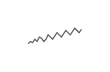
\begin{tikzpicture}[x=0.08em, y=0.08em, line width=0.4pt]
                \draw[FooterGray] (0,3) -- (1,4) -- (2,3.5) -- (3,5) -- (4,4) -- (5,6) -- (6,5.5) -- (7,4) -- (8,5) -- (9,7) -- (10,6) -- (11,5) -- (12,6.5) -- (13,8) -- (14,7) -- (15,6) -- (16,7.5) -- (17,9) -- (18,8) -- (19,7) -- (20,8.5) -- (21,10) -- (22,9) -- (23,8) -- (24,9.5);
            \end{tikzpicture}%
        }%
        \hskip0.5cm%
    }%
    \vskip6pt%
}

%=============================================================================
% PACKAGES
%=============================================================================
\usepackage[utf8]{inputenc}
\DeclareUnicodeCharacter{03B1}{\ensuremath{\alpha}}
\usepackage[T1]{fontenc}
\usepackage{amsmath, amssymb, amsthm}
\usepackage{mathtools}
\usepackage{bm}
\usepackage{tikz}
\usetikzlibrary{arrows.meta, positioning, shapes, calc, decorations.pathreplacing, shadings}
\usepackage{booktabs}
\usepackage{multirow}
\usepackage{array}
\usepackage{graphicx}
\usepackage{animate}
\usepackage{hyperref}
\usepackage{colortbl}
\usepackage{listings}
\lstset{language=Python, basicstyle=\ttfamily\scriptsize, keywordstyle=\color{MainBlue}\bfseries,
  commentstyle=\color{Forest}, stringstyle=\color{Crimson}, breaklines=true,
  frame=none, backgroundcolor=\color{VeryLightGray}, xleftmargin=2mm}
\hypersetup{colorlinks=true, linkcolor=MainBlue, urlcolor=MainBlue}
\graphicspath{{../../logos/}{../../charts/}{../../photos/}}
\usepackage{xcolor}
\hfuzz=2pt  % Suppress tiny overfull warnings (<2pt)
\vfuzz=2pt  % Suppress tiny vertical overfull warnings (<2pt)
% \mathrm in the sans-serif family of the slides (beamer resets \mathrm to the serif family at \begin{document};
% this hook runs after beamer's, so WN, Var, RMSE, ... in formulas match the surrounding text)
% Bold vectors and matrices in the same sans-serif family: \mathbf{A} in sans bold (beamer's own \mathbf came out in
% medium weight), and the bold upright Greek capitals of \boldsymbol / \bm (\bSigma, \bPhi, \boldsymbol{\Theta}) in
% cmss bold: bm.sty fixes its "boldoperators" font when it is loaded (serif cmbx), before beamer switches the
% operators to cmss, so it is reset here.
\AtBeginDocument{%
  \SetMathAlphabet{\mathrm}{normal}{\encodingdefault}{\sfdefault}{\mddefault}{n}%
  \SetMathAlphabet{\mathrm}{bold}{\encodingdefault}{\sfdefault}{bx}{n}%
  \SetMathAlphabet{\mathbf}{normal}{\encodingdefault}{\sfdefault}{bx}{n}%
  \SetMathAlphabet{\mathbf}{bold}{\encodingdefault}{\sfdefault}{bx}{n}%
  \SetSymbolFont{boldoperators}{normal}{OT1}{cmss}{bx}{n}%
  \SetSymbolFont{boldoperators}{bold}{OT1}{cmss}{bx}{n}}

%=============================================================================
% QUANTLET COMMANDS
%   \quantlet{<displayed name>}{<url>}       (generic, compatible with the older TSA decks)
%   \tsaquantlet{Ch_05}{TSA_ch5_garch}       -> https://github.com/danpele/Time-Series-Analysis/tree/main/Quantlets/Ch_05/TSA_ch5_garch
%   \qlurl{<folder>} is defined per chapter by the generator (Quantlets/Ch_NN/<folder>)
%=============================================================================
\newcommand{\tsarepo}{https://github.com/danpele/Time-Series-Analysis}
\newcommand{\tsaqlbase}{https://github.com/danpele/Time-Series-Analysis/tree/main/Quantlets}
\newcommand{\quantlet}[2]{%
    \hfill\href{#2}{%
        \raisebox{-0.15em}{
\includegraphics[height=0.7em]{ql_logo.png}}%
        \textcolor{MainBlue}{\tiny\ #1}%
    }%
}
\newcommand{\tsaquantlet}[2]{\quantlet{\detokenize{#2}}{\tsaqlbase/#1/#2}}

%=============================================================================
% NOTEBOOKS (Google Colab)
%   \colaburl{notebooks/EN/chapter5_seminar_notebook.ipynb} -> the Colab link of a file in the TSA repo
%   \nb: the chapter notebook (each seminar deck redefines it with \renewcommand)
%=============================================================================
\newcommand{\colaburl}[1]{https://colab.research.google.com/github/danpele/Time-Series-Analysis/blob/main/#1}
\newcommand{\nb}{https://colab.research.google.com/github/danpele/Time-Series-Analysis/tree/main/notebooks/EN}
\newcommand{\nbname}{notebooks/EN}

%=============================================================================
% SLIDE HELPERS (used by the generators; the same as in MFM)
%=============================================================================
% local font size for list bodies (the preamble forces \normalsize)
\newcommand{\itemsize}[1]{\setbeamertemplate{itemize/enumerate body begin}{#1}\setbeamertemplate{itemize/enumerate subbody begin}{#1}}
\newcommand{\intitle}[1]{{\hypersetup{urlcolor=white}#1}}   % white links inside coloured title bars
\newcommand{\imgcap}[1]{{\scriptsize #1}\\[0.5mm]}          % caption under a photo
\newcommand{\imgcredit}[2]{{\tiny\color{FooterGray}\href{#1}{#2}}}   % image credit: source URL, author/licence
\newcommand{\aiprompt}[1]{{\ttfamily\color{MainBlue}#1}}     % a prompt to an AI assistant

%=============================================================================
% SEMINARS: student version by default; the instructor wrapper *_solutions.tex sets \solutionstrue
%=============================================================================
\makeatletter\@ifundefined{ifsolutions}{\expandafter\newif\csname ifsolutions\endcsname}{}\makeatother
\newcommand{\solonly}[1]{\ifsolutions #1\fi}
\newcommand{\propsub}{\ifsolutions\else\framesubtitle{\ifdefined\tsalang Rezolvarea se discută la seminar\else Solution discussed in class\fi}\fi}

%=============================================================================
% APPENDIX AND CHAPTER LINKS (latex/appendix_links.py writes the calls; it also re-declares these
% macros before \begin{document}, so the decks compile with or without this preamble block)
%=============================================================================
\providecommand{\tsaapplink}[3]{\hypertarget{#2}{}\hyperlink{#1}{\beamergotobutton{#3}}}
\providecommand{\tsaappback}[2]{\begin{tikzpicture}[remember picture,overlay]\node[anchor=south east] at ([xshift=-3mm,yshift=7mm]current page.south east){\hyperlink{#1}{\beamerreturnbutton{#2}}};\end{tikzpicture}}
\providecommand{\tsachlink}[2]{\href{#1}{#2}}
\providecommand{\tsachlinkt}[2]{\href{#1}{\usebeamercolor[fg]{frametitle}#2}}

%=============================================================================
% QUANTINAR COMMAND: link către un curs Quantinar (subiecte avansate)
%=============================================================================
\newcommand{\quantinar}[2]{%
    \href{#2}{%
        \raisebox{-0.15em}{
\includegraphics[height=0.8em]{qr_logo.png}}%
        \textcolor{MainBlue}{\scriptsize\ #1}%
    }%
}

%=============================================================================
% CUSTOM TITLE PAGE
%=============================================================================
\defbeamertemplate*{title page}{hybrid}[1][]
{
    \vspace{0.2cm}
    % Logos row - top header (with clickable links)
    \begin{center}
        \href{https://www.ase.ro}{
\includegraphics[height=1.0cm]{ase_logo.png}}\hspace{0.3cm}%
        \href{https://theida.net}{
\includegraphics[height=1.0cm]{ida_logo.png}}\hspace{0.3cm}%
        \href{https://blockchain-research-center.com}{
\includegraphics[height=1.0cm]{brc_logo.png}}\hspace{0.3cm}%
        \href{https://www.ai4efin.ase.ro}{
\includegraphics[height=1.0cm]{ai4efin_logo.png}}\hspace{0.3cm}%
        \href{https://ipe.ro/new}{
\includegraphics[height=1.0cm]{acad_logo.png}}\hspace{0.3cm}%
        \href{https://www.digital-finance-msca.com}{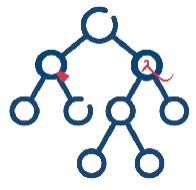
\includegraphics[height=1.0cm]{msca_logo.png}}%
    \end{center}

    \vspace{0.6cm}

    % Main title with Q logos on sides (with clickable links)
    \begin{center}
        \begin{minipage}{0.1\textwidth}
            \centering
            \href{https://quantlet.com}{
\includegraphics[height=1.1cm]{ql_logo.png}}
        \end{minipage}%
        \begin{minipage}{0.78\textwidth}
            \centering
            {\LARGE\bfseries\usebeamercolor[fg]{title}\inserttitle}

            \vspace{0.3cm}

            {\usebeamerfont{subtitle}\usebeamercolor[fg]{title}\insertsubtitle}
        \end{minipage}%
        \begin{minipage}{0.1\textwidth}
            \centering
            \href{https://quantinar.com}{
\includegraphics[height=1.1cm]{qr_logo.png}}
        \end{minipage}
    \end{center}

    \vspace{0.6cm}

    % Authors (left aligned)
    \hspace{0.5cm}{\usebeamerfont{author}\insertauthor}

    \vspace{0.3cm}

    % Institute/Affiliations (left aligned)
    \hspace{0.5cm}\begin{minipage}[t]{0.9\textwidth}
        \raggedright\small\insertinstitute
    \end{minipage}
}

%=============================================================================
% THEOREM ENVIRONMENTS
%=============================================================================
\theoremstyle{definition}
\setbeamertemplate{theorems}[numbered]
\ifdefined\tsalang
\newtheorem{defn}{Definiție}
\newtheorem{thm}{Teoremă}
\newtheorem{prop}{Propoziție}
\newtheorem{rmk}{Observație}
\else
\newtheorem{defn}{Definition}
\newtheorem{thm}{Theorem}
\newtheorem{prop}{Proposition}
\newtheorem{rmk}{Remark}
\fi

%=============================================================================
% CENTRED MINIPAGE (no extra vertical space)
%=============================================================================
\newenvironment{cminipage}[1]{%
    \par\noindent\hfill\begin{minipage}{#1}\ignorespaces
}{%
    \end{minipage}\hfill\null\par
}

%=============================================================================
% CUSTOM COMMANDS
%=============================================================================
\newcommand{\E}{\mathbb{E}}
\newcommand{\Var}{\text{Var}}
\newcommand{\Cov}{\text{Cov}}
\newcommand{\Corr}{\text{Corr}}
\newcommand{\R}{\mathbb{R}}
\newcommand{\N}{\mathbb{N}}
\newcommand{\Z}{\mathbb{Z}}
\newcommand{\B}{\mathbf{B}}
\newcommand{\imark}{\textcolor{MainBlue}{\textbullet}}
\newcommand{\RMSE}{\text{RMSE}}
\newcommand{\MAE}{\text{MAE}}
\newcommand{\MAPE}{\text{MAPE}}

% Boldface vector/matrix commands (VAR, VECM, state space; also used by the older TSA decks)
\newcommand{\bY}{\mathbf{Y}}
\newcommand{\bX}{\mathbf{X}}
\newcommand{\bA}{\mathbf{A}}
\newcommand{\bB}{\mathbf{B}}
\newcommand{\bepsilon}{\boldsymbol{\varepsilon}}
\newcommand{\bSigma}{\boldsymbol{\Sigma}}
\newcommand{\bPhi}{\boldsymbol{\Phi}}
\newcommand{\bGamma}{\boldsymbol{\Gamma}}
\newcommand{\bPi}{\boldsymbol{\Pi}}
\newcommand{\bc}{\mathbf{c}}
\newcommand{\balpha}{\boldsymbol{\alpha}}
\newcommand{\bbeta}{\boldsymbol{\beta}}
\newcommand{\bvarepsilon}{\boldsymbol{\varepsilon}}

% Legacy seminar marks (older TSA seminar decks)
\newcommand{\correct}{\textcolor{Forest}{\checkmark}}
\newcommand{\incorrect}{\textcolor{Crimson}{\texttimes}}
 se definește
%   \newcommand{\coursename}{Time Series Analysis}      (EN)
%   \newcommand{\coursename}{Serii de timp}       (RO)  și  \def\tsalang{ro}
% Fișierele .tex se află în EN/Courses, EN/Seminars, RO/Cursuri, RO/Seminarii (două niveluri sub rădăcină).
% Deck-urile sînt generate de latex/build_chapterN.py / build_seminarN.py (vezi latex/tsa_build.py).

\documentclass[9pt, aspectratio=169, t]{beamer}
\providecommand{\coursename}{Time Series Analysis}

% Ensure content fits on slides
\setbeamersize{text margin left=8mm, text margin right=8mm}
% Smaller institute font (title page)
\setbeamerfont{institute}{size=\footnotesize}

%=============================================================================
% THEME AND STYLE CONFIGURATION
%=============================================================================
\usetheme{default}
% Using default theme for clean header/footer control

% Color Palette (matching Redispatch PDF)
\definecolor{MainBlue}{RGB}{26, 58, 110}
\definecolor{AccentBlue}{RGB}{26, 58, 110}
\definecolor{IDAred}{RGB}{205, 0, 0}
\definecolor{DarkGray}{RGB}{51, 51, 51}
\definecolor{MediumGray}{RGB}{128, 128, 128}
\definecolor{LightGray}{RGB}{248, 248, 248}
\definecolor{VeryLightGray}{RGB}{235, 235, 235}
\definecolor{KeynoteGray}{RGB}{218, 218, 218}
\definecolor{SectionGray}{RGB}{120, 120, 120}
\definecolor{FooterGray}{RGB}{100, 100, 100}
\definecolor{Crimson}{RGB}{220, 53, 69}
\definecolor{Forest}{RGB}{46, 125, 50}
\definecolor{Amber}{RGB}{181, 133, 63}
\definecolor{Orange}{RGB}{230, 126, 34}
\definecolor{Purple}{RGB}{142, 68, 173}

% Gradient background (exact Keynote 315° gradient: white to RGB 218,218,218)
\setbeamertemplate{background}{%
    \begin{tikzpicture}[remember picture, overlay]
        \shade[shading=axis, shading angle=315,
        top color=white, bottom color=KeynoteGray]
        (current page.south west) rectangle (current page.north east);
    \end{tikzpicture}%
}
% Fallback solid color for compatibility
\setbeamercolor{background canvas}{bg=}

\setbeamercolor{palette primary}{bg=MainBlue, fg=white}
\setbeamercolor{palette secondary}{bg=MainBlue!85, fg=white}
\setbeamercolor{palette tertiary}{bg=MainBlue!70, fg=white}
\setbeamercolor{structure}{fg=MainBlue}
\setbeamercolor{title}{fg=IDAred}
\setbeamercolor{frametitle}{fg=IDAred, bg=}
\setbeamercolor{block title}{bg=MainBlue, fg=white}
\setbeamercolor{block body}{bg=VeryLightGray, fg=DarkGray}
\setbeamercolor{block title alerted}{bg=Crimson, fg=white}
\setbeamercolor{block body alerted}{bg=Crimson!8, fg=DarkGray}
\setbeamercolor{block title example}{bg=Forest, fg=white}
\setbeamercolor{block body example}{bg=Forest!8, fg=DarkGray}
\setbeamercolor{item}{fg=MainBlue}

% Footer colors (override Madrid theme blue)
\setbeamercolor{author in head/foot}{fg=FooterGray, bg=}
\setbeamercolor{title in head/foot}{fg=FooterGray, bg=}
\setbeamercolor{date in head/foot}{fg=FooterGray, bg=}
\setbeamercolor{section in head/foot}{fg=FooterGray, bg=}
\setbeamercolor{subsection in head/foot}{fg=FooterGray, bg=}

% Bullet styles (apply everywhere including blocks)
\setbeamertemplate{itemize item}{\color{MainBlue}$\boxdot$}
\setbeamertemplate{itemize subitem}{\color{MainBlue}$\blacktriangleright$}
\setbeamertemplate{itemize subsubitem}{\color{MainBlue}\tiny$\bullet$}
\setbeamertemplate{itemize/enumerate body begin}{\normalsize}
\setbeamertemplate{itemize/enumerate subbody begin}{\normalsize}

% Item spacing - compact style
\setlength{\leftmargini}{10pt}       % Level 1: minimal indent
\setlength{\leftmarginii}{10pt}      % Level 2: minimal additional indent
% Compact list spacing (zero extra space before/after lists in blocks)
\makeatletter
\def\@listi{\leftmargin\leftmargini \topsep 0pt \parsep 0pt \itemsep 0pt}
\def\@listii{\leftmargin\leftmarginii \topsep 0pt \parsep 0pt \itemsep 0pt}
\makeatother

\setbeamertemplate{navigation symbols}{}

%=============================================================================
% CUSTOM HEADLINE
%=============================================================================
\setbeamertemplate{headline}{%
    \vskip10pt%
    \hbox to \paperwidth{%
        \hskip0.5cm%
        {\small\color{FooterGray}\renewcommand{\hyperlink}[2]{##2}\insertsectionhead}%
        \hfill%
        \textcolor{FooterGray}{\small\insertframenumber}%
        \hskip0.5cm%
    }%
    \vskip4pt%
    {\color{FooterGray}\hrule height 0.4pt}%
}

%=============================================================================
% CUSTOM FOOTER
%=============================================================================
\usepackage{fontawesome5}

\setbeamertemplate{footline}{%
    {\color{FooterGray}\hrule height 0.4pt}%
    \vskip4pt%
    \hbox to \paperwidth{%
        \hskip0.5cm%
        \textcolor{FooterGray}{\small\coursename}%
        \hfill%
        \raisebox{-0.1em}{%
            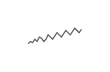
\begin{tikzpicture}[x=0.08em, y=0.08em, line width=0.4pt]
                \draw[FooterGray] (0,3) -- (1,4) -- (2,3.5) -- (3,5) -- (4,4) -- (5,6) -- (6,5.5) -- (7,4) -- (8,5) -- (9,7) -- (10,6) -- (11,5) -- (12,6.5) -- (13,8) -- (14,7) -- (15,6) -- (16,7.5) -- (17,9) -- (18,8) -- (19,7) -- (20,8.5) -- (21,10) -- (22,9) -- (23,8) -- (24,9.5);
            \end{tikzpicture}%
        }%
        \hskip0.5cm%
    }%
    \vskip6pt%
}

%=============================================================================
% PACKAGES
%=============================================================================
\usepackage[utf8]{inputenc}
\DeclareUnicodeCharacter{03B1}{\ensuremath{\alpha}}
\usepackage[T1]{fontenc}
\usepackage{amsmath, amssymb, amsthm}
\usepackage{mathtools}
\usepackage{bm}
\usepackage{tikz}
\usetikzlibrary{arrows.meta, positioning, shapes, calc, decorations.pathreplacing, shadings}
\usepackage{booktabs}
\usepackage{multirow}
\usepackage{array}
\usepackage{graphicx}
\usepackage{animate}
\usepackage{hyperref}
\usepackage{colortbl}
\usepackage{listings}
\lstset{language=Python, basicstyle=\ttfamily\scriptsize, keywordstyle=\color{MainBlue}\bfseries,
  commentstyle=\color{Forest}, stringstyle=\color{Crimson}, breaklines=true,
  frame=none, backgroundcolor=\color{VeryLightGray}, xleftmargin=2mm}
\hypersetup{colorlinks=true, linkcolor=MainBlue, urlcolor=MainBlue}
\graphicspath{{../../logos/}{../../charts/}{../../photos/}}
\usepackage{xcolor}
\hfuzz=2pt  % Suppress tiny overfull warnings (<2pt)
\vfuzz=2pt  % Suppress tiny vertical overfull warnings (<2pt)
% \mathrm in the sans-serif family of the slides (beamer resets \mathrm to the serif family at \begin{document};
% this hook runs after beamer's, so WN, Var, RMSE, ... in formulas match the surrounding text)
% Bold vectors and matrices in the same sans-serif family: \mathbf{A} in sans bold (beamer's own \mathbf came out in
% medium weight), and the bold upright Greek capitals of \boldsymbol / \bm (\bSigma, \bPhi, \boldsymbol{\Theta}) in
% cmss bold: bm.sty fixes its "boldoperators" font when it is loaded (serif cmbx), before beamer switches the
% operators to cmss, so it is reset here.
\AtBeginDocument{%
  \SetMathAlphabet{\mathrm}{normal}{\encodingdefault}{\sfdefault}{\mddefault}{n}%
  \SetMathAlphabet{\mathrm}{bold}{\encodingdefault}{\sfdefault}{bx}{n}%
  \SetMathAlphabet{\mathbf}{normal}{\encodingdefault}{\sfdefault}{bx}{n}%
  \SetMathAlphabet{\mathbf}{bold}{\encodingdefault}{\sfdefault}{bx}{n}%
  \SetSymbolFont{boldoperators}{normal}{OT1}{cmss}{bx}{n}%
  \SetSymbolFont{boldoperators}{bold}{OT1}{cmss}{bx}{n}}

%=============================================================================
% QUANTLET COMMANDS
%   \quantlet{<displayed name>}{<url>}       (generic, compatible with the older TSA decks)
%   \tsaquantlet{Ch_05}{TSA_ch5_garch}       -> https://github.com/danpele/Time-Series-Analysis/tree/main/Quantlets/Ch_05/TSA_ch5_garch
%   \qlurl{<folder>} is defined per chapter by the generator (Quantlets/Ch_NN/<folder>)
%=============================================================================
\newcommand{\tsarepo}{https://github.com/danpele/Time-Series-Analysis}
\newcommand{\tsaqlbase}{https://github.com/danpele/Time-Series-Analysis/tree/main/Quantlets}
\newcommand{\quantlet}[2]{%
    \hfill\href{#2}{%
        \raisebox{-0.15em}{
\includegraphics[height=0.7em]{ql_logo.png}}%
        \textcolor{MainBlue}{\tiny\ #1}%
    }%
}
\newcommand{\tsaquantlet}[2]{\quantlet{\detokenize{#2}}{\tsaqlbase/#1/#2}}

%=============================================================================
% NOTEBOOKS (Google Colab)
%   \colaburl{notebooks/EN/chapter5_seminar_notebook.ipynb} -> the Colab link of a file in the TSA repo
%   \nb: the chapter notebook (each seminar deck redefines it with \renewcommand)
%=============================================================================
\newcommand{\colaburl}[1]{https://colab.research.google.com/github/danpele/Time-Series-Analysis/blob/main/#1}
\newcommand{\nb}{https://colab.research.google.com/github/danpele/Time-Series-Analysis/tree/main/notebooks/EN}
\newcommand{\nbname}{notebooks/EN}

%=============================================================================
% SLIDE HELPERS (used by the generators; the same as in MFM)
%=============================================================================
% local font size for list bodies (the preamble forces \normalsize)
\newcommand{\itemsize}[1]{\setbeamertemplate{itemize/enumerate body begin}{#1}\setbeamertemplate{itemize/enumerate subbody begin}{#1}}
\newcommand{\intitle}[1]{{\hypersetup{urlcolor=white}#1}}   % white links inside coloured title bars
\newcommand{\imgcap}[1]{{\scriptsize #1}\\[0.5mm]}          % caption under a photo
\newcommand{\imgcredit}[2]{{\tiny\color{FooterGray}\href{#1}{#2}}}   % image credit: source URL, author/licence
\newcommand{\aiprompt}[1]{{\ttfamily\color{MainBlue}#1}}     % a prompt to an AI assistant

%=============================================================================
% SEMINARS: student version by default; the instructor wrapper *_solutions.tex sets \solutionstrue
%=============================================================================
\makeatletter\@ifundefined{ifsolutions}{\expandafter\newif\csname ifsolutions\endcsname}{}\makeatother
\newcommand{\solonly}[1]{\ifsolutions #1\fi}
\newcommand{\propsub}{\ifsolutions\else\framesubtitle{\ifdefined\tsalang Rezolvarea se discută la seminar\else Solution discussed in class\fi}\fi}

%=============================================================================
% APPENDIX AND CHAPTER LINKS (latex/appendix_links.py writes the calls; it also re-declares these
% macros before \begin{document}, so the decks compile with or without this preamble block)
%=============================================================================
\providecommand{\tsaapplink}[3]{\hypertarget{#2}{}\hyperlink{#1}{\beamergotobutton{#3}}}
\providecommand{\tsaappback}[2]{\begin{tikzpicture}[remember picture,overlay]\node[anchor=south east] at ([xshift=-3mm,yshift=7mm]current page.south east){\hyperlink{#1}{\beamerreturnbutton{#2}}};\end{tikzpicture}}
\providecommand{\tsachlink}[2]{\href{#1}{#2}}
\providecommand{\tsachlinkt}[2]{\href{#1}{\usebeamercolor[fg]{frametitle}#2}}

%=============================================================================
% QUANTINAR COMMAND: link către un curs Quantinar (subiecte avansate)
%=============================================================================
\newcommand{\quantinar}[2]{%
    \href{#2}{%
        \raisebox{-0.15em}{
\includegraphics[height=0.8em]{qr_logo.png}}%
        \textcolor{MainBlue}{\scriptsize\ #1}%
    }%
}

%=============================================================================
% CUSTOM TITLE PAGE
%=============================================================================
\defbeamertemplate*{title page}{hybrid}[1][]
{
    \vspace{0.2cm}
    % Logos row - top header (with clickable links)
    \begin{center}
        \href{https://www.ase.ro}{
\includegraphics[height=1.0cm]{ase_logo.png}}\hspace{0.3cm}%
        \href{https://theida.net}{
\includegraphics[height=1.0cm]{ida_logo.png}}\hspace{0.3cm}%
        \href{https://blockchain-research-center.com}{
\includegraphics[height=1.0cm]{brc_logo.png}}\hspace{0.3cm}%
        \href{https://www.ai4efin.ase.ro}{
\includegraphics[height=1.0cm]{ai4efin_logo.png}}\hspace{0.3cm}%
        \href{https://ipe.ro/new}{
\includegraphics[height=1.0cm]{acad_logo.png}}\hspace{0.3cm}%
        \href{https://www.digital-finance-msca.com}{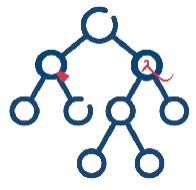
\includegraphics[height=1.0cm]{msca_logo.png}}%
    \end{center}

    \vspace{0.6cm}

    % Main title with Q logos on sides (with clickable links)
    \begin{center}
        \begin{minipage}{0.1\textwidth}
            \centering
            \href{https://quantlet.com}{
\includegraphics[height=1.1cm]{ql_logo.png}}
        \end{minipage}%
        \begin{minipage}{0.78\textwidth}
            \centering
            {\LARGE\bfseries\usebeamercolor[fg]{title}\inserttitle}

            \vspace{0.3cm}

            {\usebeamerfont{subtitle}\usebeamercolor[fg]{title}\insertsubtitle}
        \end{minipage}%
        \begin{minipage}{0.1\textwidth}
            \centering
            \href{https://quantinar.com}{
\includegraphics[height=1.1cm]{qr_logo.png}}
        \end{minipage}
    \end{center}

    \vspace{0.6cm}

    % Authors (left aligned)
    \hspace{0.5cm}{\usebeamerfont{author}\insertauthor}

    \vspace{0.3cm}

    % Institute/Affiliations (left aligned)
    \hspace{0.5cm}\begin{minipage}[t]{0.9\textwidth}
        \raggedright\small\insertinstitute
    \end{minipage}
}

%=============================================================================
% THEOREM ENVIRONMENTS
%=============================================================================
\theoremstyle{definition}
\setbeamertemplate{theorems}[numbered]
\ifdefined\tsalang
\newtheorem{defn}{Definiție}
\newtheorem{thm}{Teoremă}
\newtheorem{prop}{Propoziție}
\newtheorem{rmk}{Observație}
\else
\newtheorem{defn}{Definition}
\newtheorem{thm}{Theorem}
\newtheorem{prop}{Proposition}
\newtheorem{rmk}{Remark}
\fi

%=============================================================================
% CENTRED MINIPAGE (no extra vertical space)
%=============================================================================
\newenvironment{cminipage}[1]{%
    \par\noindent\hfill\begin{minipage}{#1}\ignorespaces
}{%
    \end{minipage}\hfill\null\par
}

%=============================================================================
% CUSTOM COMMANDS
%=============================================================================
\newcommand{\E}{\mathbb{E}}
\newcommand{\Var}{\text{Var}}
\newcommand{\Cov}{\text{Cov}}
\newcommand{\Corr}{\text{Corr}}
\newcommand{\R}{\mathbb{R}}
\newcommand{\N}{\mathbb{N}}
\newcommand{\Z}{\mathbb{Z}}
\newcommand{\B}{\mathbf{B}}
\newcommand{\imark}{\textcolor{MainBlue}{\textbullet}}
\newcommand{\RMSE}{\text{RMSE}}
\newcommand{\MAE}{\text{MAE}}
\newcommand{\MAPE}{\text{MAPE}}

% Boldface vector/matrix commands (VAR, VECM, state space; also used by the older TSA decks)
\newcommand{\bY}{\mathbf{Y}}
\newcommand{\bX}{\mathbf{X}}
\newcommand{\bA}{\mathbf{A}}
\newcommand{\bB}{\mathbf{B}}
\newcommand{\bepsilon}{\boldsymbol{\varepsilon}}
\newcommand{\bSigma}{\boldsymbol{\Sigma}}
\newcommand{\bPhi}{\boldsymbol{\Phi}}
\newcommand{\bGamma}{\boldsymbol{\Gamma}}
\newcommand{\bPi}{\boldsymbol{\Pi}}
\newcommand{\bc}{\mathbf{c}}
\newcommand{\balpha}{\boldsymbol{\alpha}}
\newcommand{\bbeta}{\boldsymbol{\beta}}
\newcommand{\bvarepsilon}{\boldsymbol{\varepsilon}}

% Legacy seminar marks (older TSA seminar decks)
\newcommand{\correct}{\textcolor{Forest}{\checkmark}}
\newcommand{\incorrect}{\textcolor{Crimson}{\texttimes}}


\newcommand{\qlurl}[1]{https://github.com/danpele/Time-Series-Analysis/tree/main/Quantlets/Ch_10/#1}

% Clickable citations (DOIs verified via Crossref)
\newcommand{\refHP}{\href{https://doi.org/10.1007/978-3-031-13584-2}{Huang and Petukhina (2022)}}
\newcommand{\refDK}{\href{https://doi.org/10.1093/acprof:oso/9780199641178.001.0001}{Durbin and Koopman (2012)}}
\newcommand{\refHarvey}{\href{https://doi.org/10.1017/CBO9781107049994}{Harvey (1989)}}
\newcommand{\refHamilton}{\href{https://doi.org/10.2307/j.ctv14jx6sm}{Hamilton (1994)}}
\newcommand{\refKN}{\href{https://doi.org/10.7551/mitpress/6444.001.0001}{Kim and Nelson (1999)}}
\newcommand{\refSS}{\href{https://doi.org/10.1007/978-3-319-52452-8}{Shumway and Stoffer (2017)}}
\newcommand{\refKalman}{\href{https://doi.org/10.1115/1.3662552}{Kalman (1960)}}
\newcommand{\refRTS}{\href{https://doi.org/10.2514/3.3166}{Rauch, Tung and Striebel (1965)}}
\newcommand{\refMuth}{\href{https://doi.org/10.1080/01621459.1960.10482064}{Muth (1960)}}
\newcommand{\refHKOS}{\href{https://doi.org/10.1007/978-3-540-71918-2}{Hyndman et al.\ (2008)}}
\newcommand{\refHJ}{\href{https://doi.org/10.1002/jae.3950080302}{Harvey and Jaeger (1993)}}
\newcommand{\refHPf}{\href{https://doi.org/10.2307/2953682}{Hodrick and Prescott (1997)}}
\newcommand{\refHamHP}{\href{https://doi.org/10.1162/rest\_a\_00706}{Hamilton (2018)}}
\newcommand{\refSW}{\href{https://doi.org/10.1086/654119}{Stock and Watson (1989)}}
\newcommand{\refGRS}{\href{https://doi.org/10.1016/j.jmoneco.2008.05.010}{Giannone, Reichlin and Small (2008)}}
\newcommand{\refHamMS}{\href{https://doi.org/10.2307/1912559}{Hamilton (1989)}}
\newcommand{\refHamEM}{\href{https://doi.org/10.1016/0304-4076(90)90093-9}{Hamilton (1990)}}
\newcommand{\refKim}{\href{https://doi.org/10.1016/0304-4076(94)90036-1}{Kim (1994)}}
\newcommand{\refCP}{\href{https://doi.org/10.1198/073500107000000296}{Chauvet and Piger (2008)}}
\newcommand{\refHSus}{\href{https://doi.org/10.1016/0304-4076(94)90067-1}{Hamilton and Susmel (1994)}}
\newcommand{\refLL}{\href{https://doi.org/10.1080/07350015.1990.10509794}{Lamoureux and Lastrapes (1990)}}
\newcommand{\refDI}{\href{https://doi.org/10.1016/S0304-4076(01)00073-2}{Diebold and Inoue (2001)}}

\title[Time Series Analysis]{Time Series Analysis}
\subtitle{Chapter 10: State space models, Kalman filter and Markov switching}
\author[D.T. Pele]{Daniel Traian PELE}
\institute{Bucharest University of Economic Studies\\
IDA Institute Digital Assets\\
Blockchain Research Center\\
AI4EFin Artificial Intelligence for Energy Finance\\
Romanian Academy, Institute for Economic Forecasting\\
MSCA Digital Finance}
\date{}

%=============================================================================
\providecommand{\tsaapplink}[3]{\hypertarget{#2}{}\hyperlink{#1}{\beamergotobutton{#3}}}  % APPLINKS-MACROS
\providecommand{\tsaappback}[2]{\begin{tikzpicture}[remember picture,overlay]\node[anchor=south east] at ([xshift=-3mm,yshift=7mm]current page.south east){\hyperlink{#1}{\beamerreturnbutton{#2}}};\end{tikzpicture}}  % APPLINKS-MACROS
\providecommand{\tsachlink}[2]{\href{#1}{#2}}  % APPLINKS-MACROS
\providecommand{\tsachlinkt}[2]{\href{#1}{\usebeamercolor[fg]{frametitle}#2}}  % APPLINKS-MACROS
\begin{document}
%=============================================================================

{
\setbeamertemplate{headline}{}
\setbeamertemplate{footline}{}
\begin{frame}[noframenumbering]
    \titlepage
\end{frame}
}
% BEGIN-ACRONYMS (generat de latex/acronyms.py; nu editati manual)
\begin{frame}{Acronyms used in this material (1/2)}
\setbeamertemplate{itemize/enumerate body begin}{\tiny}
\begin{columns}[T]
\begin{column}{0.49\textwidth}
\begin{itemize}\setlength{\itemsep}{0pt}
    \item \textbf{ACF}: Autocorrelation Function
    \item \textbf{AI}: Artificial Intelligence
    \item \textbf{AIC}: Akaike Information Criterion
    \item \textbf{AR}: AutoRegressive (model); in event studies: Abnormal Return
    \item \textbf{ARCH}: AutoRegressive Conditional Heteroskedasticity
    \item \textbf{ARIMA}: AutoRegressive Integrated Moving Average (model)
    \item \textbf{ARMA}: AutoRegressive Moving Average (model)
    \item \textbf{BET}: Bucharest Exchange Trading (index)
    \item \textbf{BIC}: Bayesian Information Criterion
    \item \textbf{EM}: Expectation–Maximisation (algorithm)
    \item \textbf{EODHD}: EOD Historical Data (market-data provider)
    \item \textbf{ETS}: Error, Trend, Seasonality (exponential smoothing state space models)
    \item \textbf{EU}: European Union
\end{itemize}
\end{column}
\begin{column}{0.49\textwidth}
\begin{itemize}\setlength{\itemsep}{0pt}
    \item \textbf{FRED}: Federal Reserve Economic Data
    \item \textbf{GARCH}: Generalised AutoRegressive Conditional Heteroskedasticity
    \item \textbf{GDP}: Gross Domestic Product
    \item \textbf{GDPC1}: Real Gross Domestic Product, chained dollars (FRED series code)
    \item \textbf{HP}: Hodrick–Prescott (filter)
    \item \textbf{MA}: Moving Average
    \item \textbf{ML}: Machine Learning
    \item \textbf{MS-AR}: Markov-Switching AutoRegressive (model)
    \item \textbf{NASA}: National Aeronautics and Space Administration
    \item \textbf{NBER}: National Bureau of Economic Research
    \item \textbf{OLS}: Ordinary Least Squares
    \item \textbf{RTS}: Rauch–Tung–Striebel (smoother)
    \item \textbf{SD}: Standard Deviation
\end{itemize}
\end{column}
\end{columns}
\end{frame}
\begin{frame}{Acronyms used in this material (2/2)}
\setbeamertemplate{itemize/enumerate body begin}{\tiny}
\begin{columns}[T]
\begin{column}{0.49\textwidth}
\begin{itemize}\setlength{\itemsep}{0pt}
    \item \textbf{SES}: Simple Exponential Smoothing
    \item \textbf{SWARCH}: Switching ARCH
    \item \textbf{TVP}: Time-Varying Parameter (regression)
    \item \textbf{UC}: Unobserved Components (model)
    \item \textbf{US}: United States
    \item \textbf{USREC}: US Recession indicator (FRED series code)
    \item \textbf{VAR}: Vector AutoRegression
\end{itemize}
\end{column}
\begin{column}{0.49\textwidth}
\end{column}
\end{columns}
\end{frame}
% END-ACRONYMS

\begin{frame}{Today's question and route}
\itemsize{\small}
\begin{itemize}
    \item \textbf{Question}: how do we measure what we cannot observe directly: the true level of a noisy series, the output gap, a changing beta, a recession?
    \begin{itemize}
        \item the answer: write the unobserved quantity as a \textbf{state} and let the data update our estimate of it, period by period
    \end{itemize}
    \item \textbf{Route} of the chapter
    \begin{itemize}
        \item the state space form: measurement and transition equations; local level, local linear trend, ARMA, time-varying regression
        \item the Kalman filter by hand; smoothing; likelihood and estimation; missing values
        \item trend and cycle: Romanian GDP, the HP filter and its critique; dynamic factors and nowcasting
        \item Markov switching: recessions, Romanian growth regimes, volatility regimes
    \end{itemize}
    \item We build on \tsachlink{https://danpele.github.io/Time-Series-Analysis/EN/Courses/chapter0_introduction.pdf}{Chapter 0} (exponential smoothing), \tsachlink{https://danpele.github.io/Time-Series-Analysis/EN/Courses/chapter2_arma_models.pdf}{Chapter 2} (ARMA), \tsachlink{https://danpele.github.io/Time-Series-Analysis/EN/Courses/chapter5_conditional_volatility_garch.pdf}{Chapter 5} (GARCH) and \tsachlink{https://danpele.github.io/Time-Series-Analysis/EN/Courses/chapter8_long_memory_arfima.pdf}{Chapter 8} (long memory); Seminar 10 comes before this lecture
\end{itemize}
\end{frame}

\begin{frame}{Learning outcomes}
\itemsize{\small}
\begin{itemize}
    \item Write a model in state space form: local level, local linear trend, AR(2), a regression with a time-varying coefficient
    \item Run the Kalman filter by hand and explain the Kalman gain
    \item Show that simple exponential smoothing is the steady state of the local level filter
    \item Estimate a state space model by maximum likelihood, smooth it, and handle missing values and forecasts
    \item Decompose GDP into trend and cycle and judge the HP filter against the critique of Hamilton (2018)
    \item Estimate a Markov-switching model and read its regime probabilities, durations and pitfalls
\end{itemize}
\end{frame}

\begin{frame}{Reading and tools}
\itemsize{\small}
\begin{itemize}
    \item Textbook: \refHP, the chapter on state space models and the Kalman filter
    \begin{itemize}
        \item state space: \refDK\ (the Nile example of this chapter comes from their book); \refHarvey; \refSS, Ch.~6
        \item regime switching: \refHamMS; \refHamilton, Ch.~13 (Kalman filter) and Ch.~22 (regime changes); \refKN
    \end{itemize}
    \item Python Quantlets of this chapter: \href{https://github.com/danpele/Time-Series-Analysis/tree/main/Quantlets/Ch_10}{Quantlets/Ch\_10}
    \begin{itemize}
        \item a Kalman filter written out in \texttt{numpy}; \texttt{statsmodels}: \texttt{UnobservedComponents}, \texttt{SARIMAX}, \texttt{DynamicFactor}, \texttt{MarkovRegression}, \texttt{MarkovAutoregression}
    \end{itemize}
    \item Lecture notebook: \href{\colaburl{notebooks/EN/chapter10_lecture_notebook.ipynb}}{open in Google Colab}
    \item Video course: \quantinar{Kalman Filter}{https://quantinar.com/course/42/methodology}
\end{itemize}
\end{frame}


%=============================================================================
\section{Hidden states}
%=============================================================================

\begin{frame}{Rudolf Kálmán and the Apollo navigation}
\itemsize{\footnotesize}
\begin{columns}[T]
\begin{column}{0.4\textwidth}
\centering
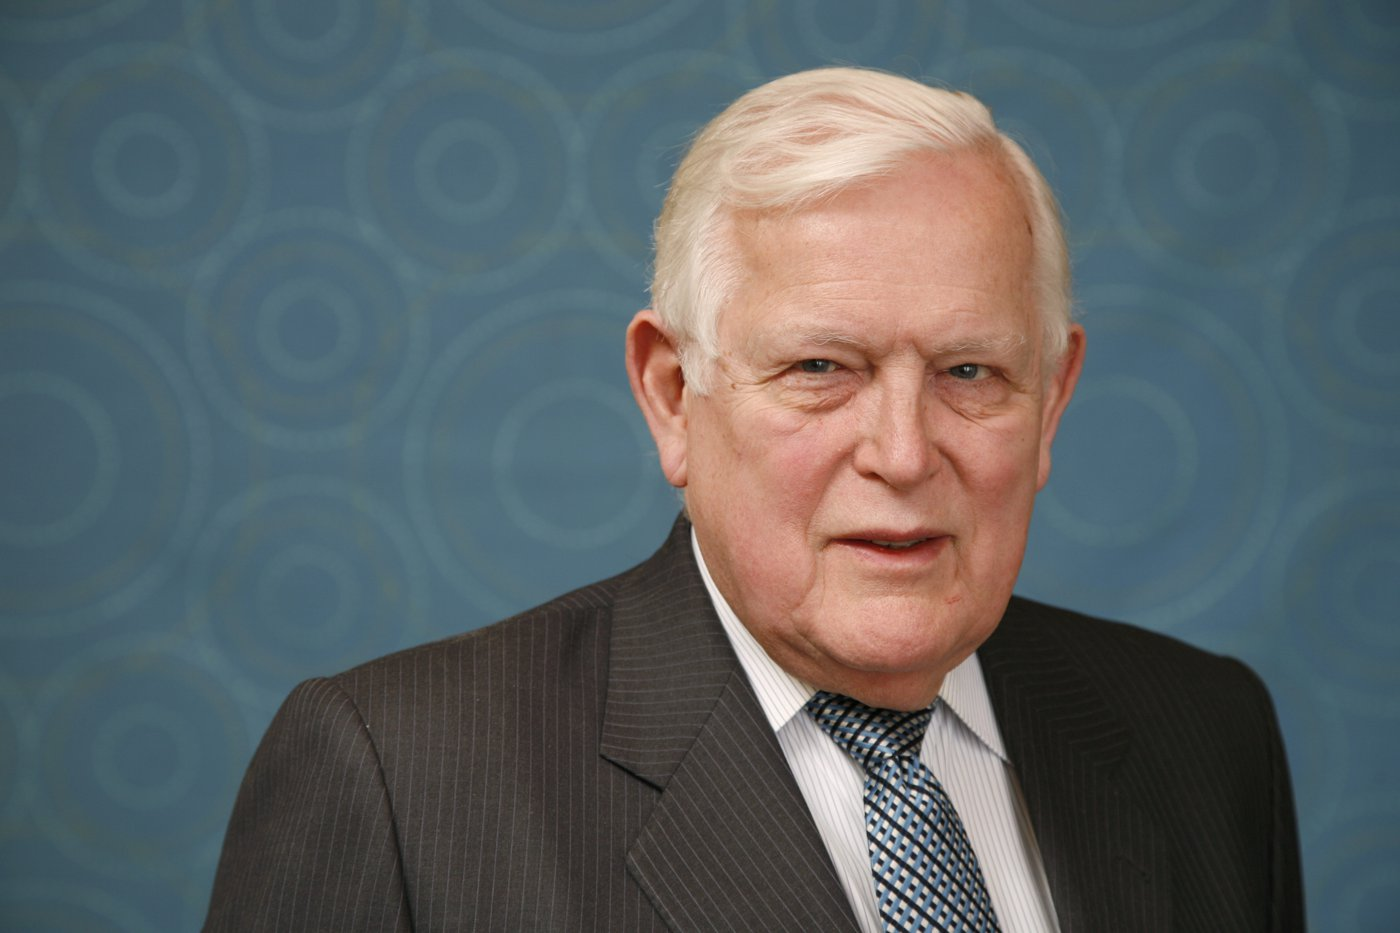
\includegraphics[height=0.25\textheight]{ch10_kalman_2007.jpg}\\[1mm]
\imgcap{Rudolf E. Kálmán (1930--2016)}
\imgcredit{https://commons.wikimedia.org/wiki/File:ETH-BIB-Kalman,_Rudolf_E._(1930-2016)-HK_04-01925.jpg}{Photo: ETH-Bibliothek Zürich, Bildarchiv (2007); CC BY-SA 4.0; Wikimedia Commons}\\[1mm]\centering
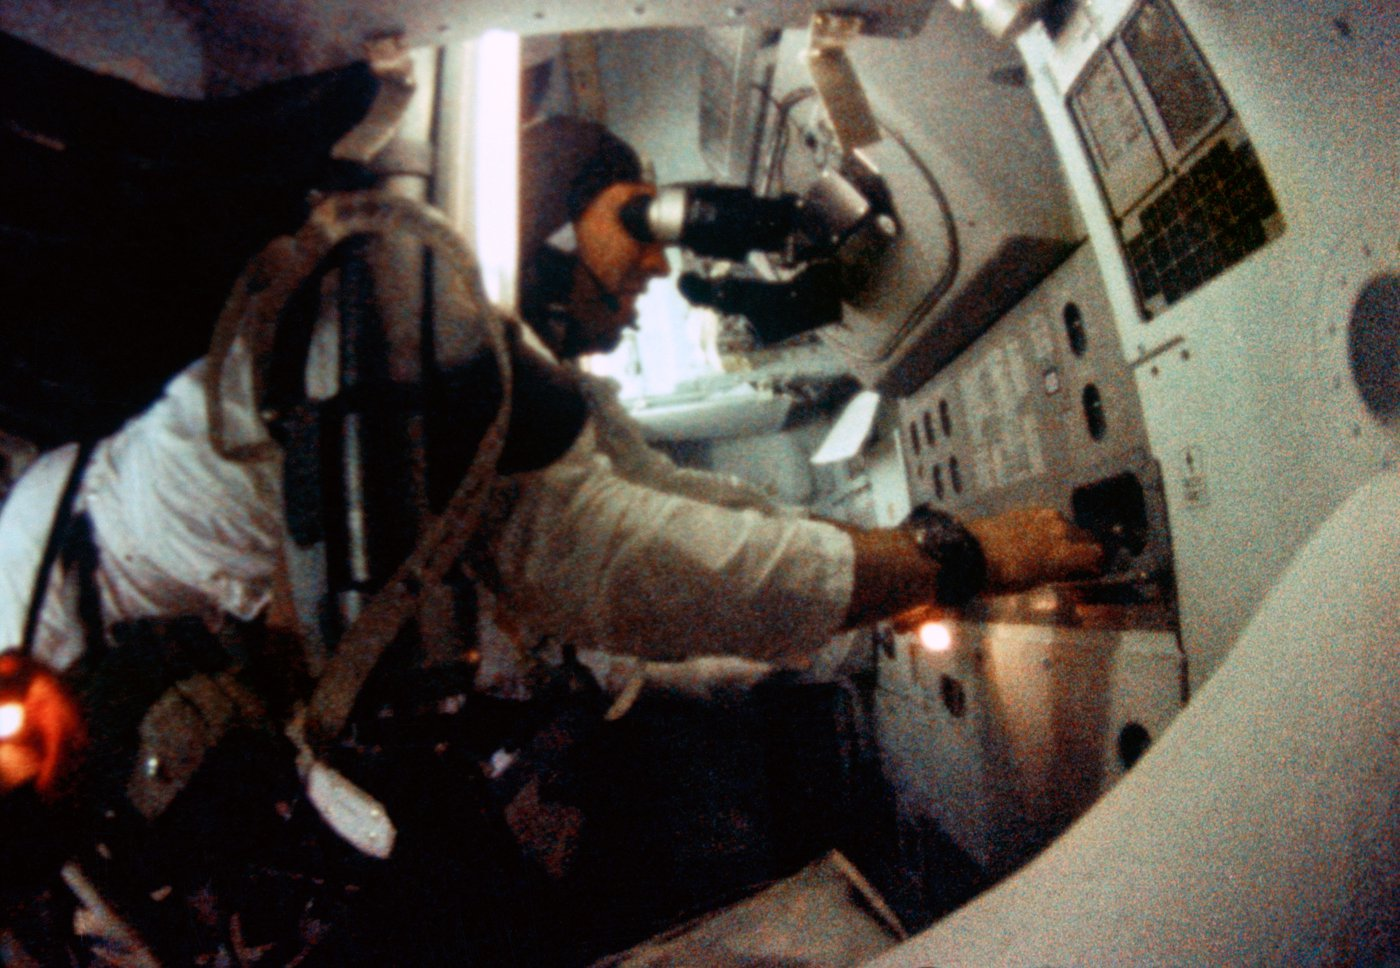
\includegraphics[height=0.21\textheight]{ch10_apollo8_navigation_1968.jpg}\\[1mm]
\imgcap{Apollo 8 (1968): Jim Lovell at the guidance and navigation station}
\imgcredit{https://commons.wikimedia.org/wiki/File:Apollo_8_Lovell_at_Guidance_and_Navigation_station.jpg}{Photo: NASA (1968); public domain; Wikimedia Commons}
\end{column}
\begin{column}{0.58\textwidth}
\begin{itemize}
    \item \refKalman: a recursive estimate of a hidden state from noisy measurements
    \begin{itemize}
        \item at each step: predict the state, then correct the prediction with the new measurement
        \item the correction weight, the \textbf{Kalman gain}, balances the two sources of uncertainty
    \end{itemize}
    \item The filter was adapted at NASA Ames for the navigation of the Apollo spacecraft
    \begin{itemize}
        \item state: position and velocity; measurements: star sightings and radar
    \end{itemize}
    \item In economics the state is a trend, a cycle, a coefficient or a regime; the measurements are the published data
\end{itemize}
\end{column}
\end{columns}
\end{frame}

\begin{frame}{Hidden states in economics and finance}
\itemsize{\small}
\begin{center}
\footnotesize
\begin{tabular}{>{\raggedright\arraybackslash}p{3.6cm}>{\raggedright\arraybackslash}p{3.6cm}>{\raggedright\arraybackslash}p{3.4cm}}
\toprule
\textbf{Observed series} & \textbf{Hidden state} & \textbf{Model in this chapter} \\
\midrule
Nile flow, monthly inflation & the underlying level & local level \\
real GDP & trend and output gap & unobserved components \\
stock index returns & a time-varying beta & time-varying regression \\
several activity indicators & one common factor & dynamic factor model \\
GDP growth, returns & recession or expansion; calm or turbulent & Markov switching \\
\bottomrule
\end{tabular}
\end{center}
\begin{itemize}
    \item The first four have a \textbf{continuous} state and are filtered by the Kalman filter
    \item The last has a \textbf{discrete} state (a regime) and is filtered by the Hamilton filter
    \item Both filters do the same thing: predict the state, then update the prediction with $y_t$
\end{itemize}
\end{frame}


%=============================================================================
\section{The state space form}
%=============================================================================

\begin{frame}{The state space form}
\itemsize{\small}
\begin{itemize}
    \item \textbf{Measurement equation}: $y_t = Z_t\alpha_t + \varepsilon_t$, \quad $\varepsilon_t \sim N(0, H)$
    \begin{itemize}
        \item $y_t$: the observation (here a scalar); $\alpha_t$: the \textbf{state vector} ($m \times 1$), not observed; $Z_t$: a $1 \times m$ row of known numbers
    \end{itemize}
    \item \textbf{Transition equation}: $\alpha_{t+1} = T\alpha_t + R\eta_t$, \quad $\eta_t \sim N(0, Q)$
    \begin{itemize}
        \item the state evolves as a first-order vector autoregression (VAR(1), \tsachlink{https://danpele.github.io/Time-Series-Analysis/EN/Courses/chapter6_var_models_granger_causality.pdf}{Chapter 6}); $T$ is $m \times m$
        \item $R$: maps the shocks $\eta_t$ into the state; $H$, $Q$: the variances of the measurement and of the state shocks
        \item initial state: $\alpha_1 \sim N(a_1, P_1)$, $a_1$, $P_1$: its mean and variance; $\varepsilon_t$, $\eta_s$ and $\alpha_1$ mutually independent
    \end{itemize}
    \item The \textbf{system matrices} $Z_t, H, T, R, Q$ contain the parameters $\theta$; they are estimated by maximum likelihood
    \begin{itemize}
        \item the same form covers ARMA, exponential smoothing, trend--cycle models, regressions with moving coefficients and factor models \refDK
    \end{itemize}
\end{itemize}
\end{frame}

\begin{frame}{The local level model}
\itemsize{\small}
\begin{itemize}
    \item \textbf{Local level} (random walk plus noise): $y_t = \mu_t + \varepsilon_t$, \quad $\mu_{t+1} = \mu_t + \eta_t$
    \begin{itemize}
        \item state $\alpha_t = \mu_t$, the level; $Z = T = R = 1$, $H = \sigma^2_\varepsilon$, $Q = \sigma^2_\eta$
        \item $\varepsilon_t$: measurement noise that disappears next period; $\eta_t$: a permanent shift of the level
    \end{itemize}
    \item \textbf{Signal-to-noise ratio} $q = \sigma^2_\eta/\sigma^2_\varepsilon$: how much of the movement is permanent
    \begin{itemize}
        \item $q = 0$: a constant level (white noise around a mean); $q \to \infty$: a pure random walk
    \end{itemize}
    \item Reduced form: $\Delta y_t = \eta_{t-1} + \varepsilon_t - \varepsilon_{t-1}$ is an MA(1) with $\rho(1) = -1/(q+2)$
    \begin{itemize}
        \item so the local level model is an ARIMA(0,1,1) (\tsachlink{https://danpele.github.io/Time-Series-Analysis/EN/Courses/chapter3_unit_roots_arima_models.pdf}{Chapter 3}) with a negative MA coefficient
        \item $\gamma(0) = \sigma^2_\eta + 2\sigma^2_\varepsilon$ and $\gamma(1) = -\sigma^2_\varepsilon$ give $\rho(1)$
    \end{itemize}
\end{itemize}
\end{frame}

\begin{frame}{Local level and local linear trend paths}
\itemsize{\footnotesize}
\begin{center}
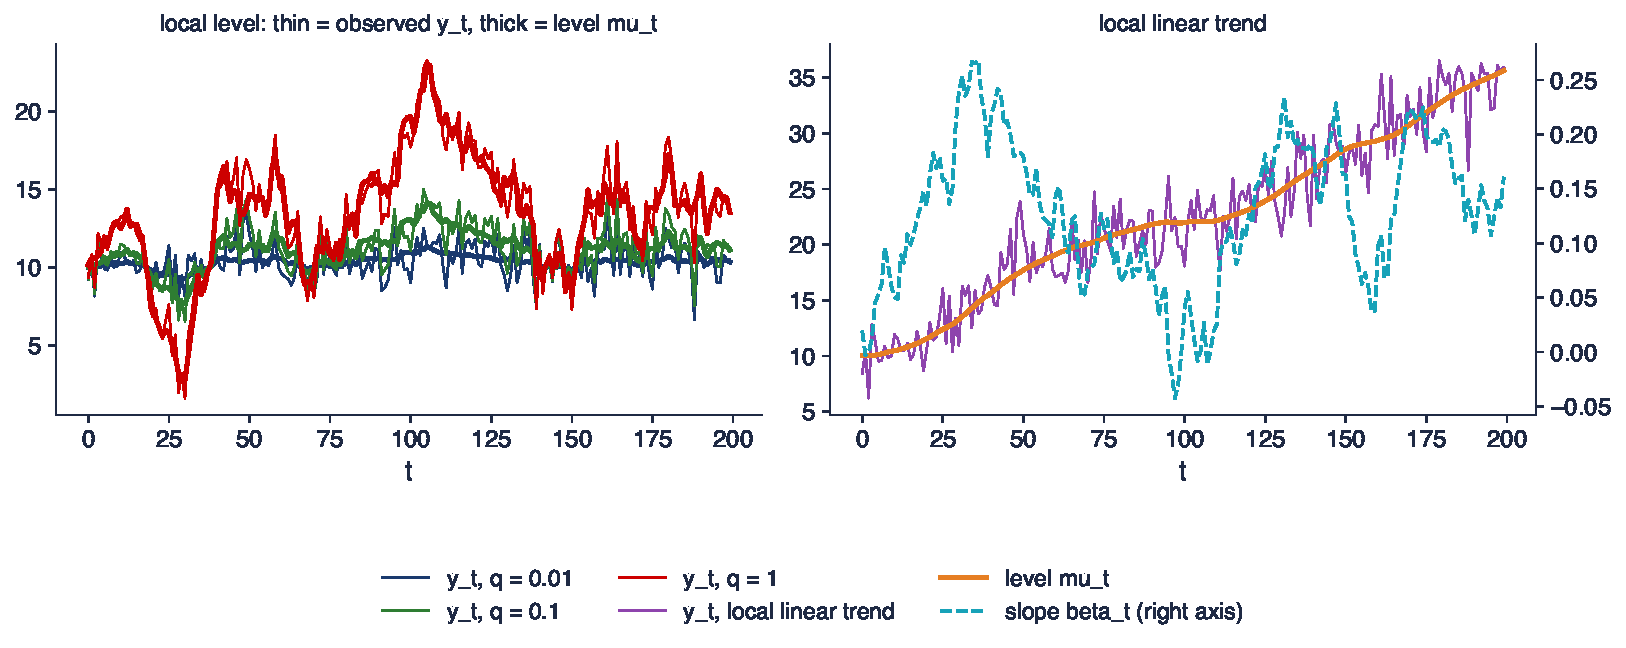
\includegraphics[width=0.97\textwidth,height=0.66\textheight,keepaspectratio]{tsa_ch10_ss_examples.pdf}
\end{center}
\vspace{-0.25cm}
\begin{itemize}
    \item Left: the same shocks $\varepsilon_t, \eta_t \sim N(0, 1)$ with $\sigma^2_\varepsilon = 1$ and $q = 0.01;\ 0.1;\ 1$ (thin: $y_t$, thick: $\mu_t$). Right: a local linear trend, whose slope $\beta_t$ is itself a random walk
\end{itemize}
\quantlet{TSA\_ch10\_state\_space\_examples}{\qlurl{TSA_ch10_state_space_examples}}
\end{frame}

\begin{frame}{Interpreting the simulated paths}
\itemsize{\small}
\begin{itemize}
    \item Small $q$: the level hardly moves and $y_t$ looks like noise around a mean; large $q$: the level wanders and $y_t$ follows it
    \begin{itemize}
        \item first-difference autocorrelation: \ensuremath{-}0.51 for $q = 0.01$ (theory $-1/2.01$) and \ensuremath{-}0.28 for $q = 1$ (theory $-1/3$)
    \end{itemize}
    \item The local linear trend has a slope that changes slowly: periods of fast and slow growth
    \begin{itemize}
        \item this is the trend model we will use for GDP
    \end{itemize}
    \item The estimation problem: from $y_t$ alone, how much is level and how much is noise? The Kalman filter answers it for given variances; the likelihood chooses the variances
\end{itemize}
\end{frame}

\begin{frame}{The local linear trend}
\itemsize{\small}
\begin{itemize}
    \item \textbf{Local linear trend}: $y_t = \mu_t + \varepsilon_t$, \quad $\mu_{t+1} = \mu_t + \beta_t + \eta_t$, \quad $\beta_{t+1} = \beta_t + \zeta_t$
    \begin{itemize}
        \item state $\alpha_t = (\mu_t, \beta_t)'$: the level and the slope (the growth rate)
        \item $Z = (1,\ 0)$, \quad $T = \begin{pmatrix}1 & 1\\ 0 & 1\end{pmatrix}$, \quad $Q = \mathrm{diag}(\sigma^2_\eta, \sigma^2_\zeta)$
    \end{itemize}
    \item Special cases
    \begin{itemize}
        \item $\sigma^2_\eta = \sigma^2_\zeta = 0$: a deterministic linear trend $\mu_1 + \beta_1 t$ (\tsachlink{https://danpele.github.io/Time-Series-Analysis/EN/Courses/chapter3_unit_roots_arima_models.pdf}{Chapter 3})
        \item $\sigma^2_\zeta = 0$: a random walk with drift $\beta$
        \item $\sigma^2_\eta = 0$: the \textbf{smooth trend} (integrated random walk), the model behind the HP filter (Section 5)
    \end{itemize}
    \item Forecasts: $\hat y_{T+h} = \hat\mu_T + h\hat\beta_T$, the state space version of Holt's method (\tsachlink{https://danpele.github.io/Time-Series-Analysis/EN/Courses/chapter0_introduction.pdf}{Chapter 0})
\end{itemize}
\end{frame}

\begin{frame}{ARMA models in state space form}
\itemsize{\small}
\begin{itemize}
    \item \textbf{AR(2)}: $y_t = \phi_1y_{t-1} + \phi_2y_{t-2} + u_t$; state $\alpha_t = (y_t, y_{t-1})'$
    \begin{itemize}
        \item $y_t = (1,\ 0)\,\alpha_t$ ($H = 0$), \quad $\alpha_{t+1} = \begin{pmatrix}\phi_1 & \phi_2\\ 1 & 0\end{pmatrix}\alpha_t + \begin{pmatrix}1\\ 0\end{pmatrix}u_{t+1}$
        \item $T$ is the companion matrix of \tsachlink{https://danpele.github.io/Time-Series-Analysis/EN/Courses/chapter2_arma_models.pdf}{Chapter 2}; its eigenvalues are the inverse AR roots
    \end{itemize}
    \item \textbf{ARMA(1,1)}: $y_t = \phi y_{t-1} + u_t + \theta u_{t-1}$ with $\alpha_t = (y_t, \theta u_t)'$
    \begin{itemize}
        \item $T = \begin{pmatrix}\phi & 1\\ 0 & 0\end{pmatrix}$, $R = (1,\ \theta)'$; any ARMA$(p,q)$ fits with $m = \max(p, q+1)$
    \end{itemize}
    \item Why it matters: the Kalman filter gives the \textbf{exact} Gaussian likelihood of an ARMA model, with missing values allowed
    \begin{itemize}
        \item the stationary start: $P_1$ solves $P = TPT' + RQR'$, i.e.\ $\mathrm{vec}(P_1) = (I - T \otimes T)^{-1}\mathrm{vec}(RQR')$
        \item this is how \texttt{statsmodels} \texttt{SARIMAX} estimates the ARIMA models of \tsachlink{https://danpele.github.io/Time-Series-Analysis/EN/Courses/chapter2_arma_models.pdf}{Chapters 2}--\tsachlink{https://danpele.github.io/Time-Series-Analysis/EN/Courses/chapter4_seasonality_forecasting.pdf}{4}
    \end{itemize}
\end{itemize}
\end{frame}

\begin{frame}{Worked example: AR(2) for US GDP growth}
\itemsize{\small}
\begin{itemize}
    \item Data: US real GDP growth, quarter on quarter, 1947--2019 ($T = 291$, FRED GDPC1)
    \begin{itemize}
        \item AR(2) with a constant by \texttt{SARIMAX}: $\hat\phi_1 = 0.319$, $\hat\phi_2 = 0.111$, $\hat\sigma^2 = 0.739$, mean $\hat\mu = 0.774\%$ per quarter
    \end{itemize}
    \item Our own filter, with the state space matrices of the previous slide and the stationary $P_1$
    \begin{itemize}
        \item log-likelihood: Kalman \ensuremath{-}368.9157; \texttt{SARIMAX} \ensuremath{-}368.9157: the same number
    \end{itemize}
    \item The prediction errors $v_t$ of the filter are the one-step forecast errors of the AR(2); the likelihood is built from them (Section 4)
\end{itemize}
\end{frame}

\begin{frame}{Regression with time-varying parameters}
\itemsize{\small}
\begin{itemize}
    \item \textbf{Time-varying parameter (TVP) regression}: $y_t = \alpha + \beta_t x_t + \varepsilon_t$, \quad $\beta_{t+1} = \beta_t + \eta_t$
    \begin{itemize}
        \item state $(\alpha, \beta_t)'$; the row $Z_t = (1,\ x_t)$ \textbf{changes over time}; $Q = \mathrm{diag}(0, \sigma^2_\eta)$
        \item $\sigma^2_\eta = 0$: ordinary least squares (OLS), computed recursively
    \end{itemize}
    \item Examples
    \begin{itemize}
        \item a market beta that rises in crises; the pass-through of the exchange rate to inflation; the persistence of inflation
    \end{itemize}
    \item Better than a rolling window: no window length to choose, every observation is used, and $\beta_t$ comes with a standard error
\end{itemize}
\end{frame}

\begin{frame}{Exponential smoothing as a state space model}
\itemsize{\small}
\begin{itemize}
    \item \tsachlink{https://danpele.github.io/Time-Series-Analysis/EN/Courses/chapter0_introduction.pdf}{Chapter 0}: simple exponential smoothing (SES) updates a level $\ell_t = \alpha y_t + (1-\alpha)\ell_{t-1}$ and forecasts $\hat y_{t+1} = \ell_t$
    \begin{itemize}
        \item equivalently $\ell_t = \ell_{t-1} + \alpha(y_t - \ell_{t-1})$: old level plus a share $\alpha$ of the surprise
    \end{itemize}
    \item \refMuth: SES gives the optimal forecasts when the data follow the local level model
    \begin{itemize}
        \item Section 3 shows it: $\alpha$ is the steady-state Kalman gain
    \end{itemize}
    \item ETS models (error, trend, seasonal) are state space models with a single source of error \refHKOS; the models here have separate shocks for each component
\end{itemize}
\end{frame}

\begin{frame}{Recap: The state space form}
\itemsize{\small}
\begin{itemize}
    \item $y_t = Z_t\alpha_t + \varepsilon_t$, $\alpha_{t+1} = T\alpha_t + R\eta_t$: a hidden VAR(1) observed with noise
    \item Local level: $q = \sigma^2_\eta/\sigma^2_\varepsilon$; reduced form ARIMA(0,1,1)
    \item Local linear trend, ARMA and TVP regression are other choices of $Z_t, T, Q$
    \item The Kalman likelihood of an AR(2) equals the exact ARMA likelihood
\end{itemize}
\end{frame}


%=============================================================================
\section{The Kalman filter}
%=============================================================================

\begin{frame}{The idea of the filter}
\itemsize{\small}
\begin{itemize}
    \item Notation: $Y_t = (y_1, \dots, y_t)$; we track two numbers (vectors) for the state
    \begin{itemize}
        \item prediction: $a_t = E(\alpha_t \mid Y_{t-1})$ with variance $P_t$
        \item filtered estimate: $a_{t|t} = E(\alpha_t \mid Y_t)$ with variance $P_{t|t}$
    \end{itemize}
    \item Each period has two steps
    \begin{itemize}
        \item \textbf{update}: $y_t$ arrives; correct $a_t$ by a share of the surprise $v_t = y_t - Z_ta_t$
        \item \textbf{prediction}: push the filtered state through the transition equation to get $a_{t+1}$
    \end{itemize}
    \item With Gaussian errors, $a_{t|t}$ is the exact conditional mean; without normality it is still the best \textbf{linear} estimate \refDK
    \item Start: $a_1, P_1$; for a non-stationary state we use a \textbf{diffuse} start ($P_1$ very large: we know nothing)
\end{itemize}
\end{frame}

\begin{frame}{The two steps in formulas}
\itemsize{\small}
\begin{itemize}
    \item \textbf{Update} (when $y_t$ is observed)
    \begin{itemize}
        \item prediction error $v_t = y_t - Z_ta_t$, with variance $F_t = Z_tP_tZ_t' + H$
        \item \textbf{Kalman gain} $K_t = P_tZ_t'F_t^{-1}$
        \item $a_{t|t} = a_t + K_tv_t$, \quad $P_{t|t} = P_t - K_tZ_tP_t$
    \end{itemize}
    \item \textbf{Prediction}
    \begin{itemize}
        \item $a_{t+1} = Ta_{t|t}$, \quad $P_{t+1} = TP_{t|t}T' + RQR'$
    \end{itemize}
    \item \textbf{Local level}: $F_t = P_t + \sigma^2_\varepsilon$, \quad $K_t = P_t/(P_t + \sigma^2_\varepsilon)$
    \begin{itemize}
        \item $a_{t+1} = a_t + K_t(y_t - a_t)$, \quad $P_{t+1} = P_t(1 - K_t) + \sigma^2_\eta$
    \end{itemize}
    \item Missing $y_t$: skip the update ($a_{t|t} = a_t$, $P_{t|t} = P_t$) and predict
\end{itemize}
\end{frame}

\begin{frame}{The Kalman gain}
\itemsize{\small}
\begin{itemize}
    \item Local level: $K_t = \dfrac{P_t}{P_t + \sigma^2_\varepsilon}$ is the weight of the new observation, between 0 and 1
    \begin{itemize}
        \item $a_{t|t} = (1 - K_t)\,a_t + K_t\,y_t$: a weighted average of the prediction and the observation
    \end{itemize}
    \item Two uncertainties compete
    \begin{itemize}
        \item noisy measurements (large $\sigma^2_\varepsilon$): small $K_t$, trust the model
        \item uncertain state (large $P_t$, e.g.\ at the start or after missing data): large $K_t$, trust the data
    \end{itemize}
    \item The variance always falls with an observation: $P_{t|t} = (1 - K_t)P_t \le P_t$
    \begin{itemize}
        \item and grows by $\sigma^2_\eta$ in the prediction step: the two forces settle at a steady state
    \end{itemize}
    \item The same formula as the weighting of two independent estimates by their precisions $1/P_t$ and $1/\sigma^2_\varepsilon$
\end{itemize}
\end{frame}

\begin{frame}{Worked example: three periods by hand (1/2)}
\itemsize{\small}
\begin{itemize}
    \item Local level with $\sigma^2_\varepsilon = 4$, $\sigma^2_\eta = 1$ ($q = 0.25$); prior $a_1 = 10$, $P_1 = 4$; data $y = (12, 11, 14)$
    \begin{itemize}
        \item $t = 1$: $F_1 = 4 + 4 = 8$, $K_1 = 4/8 = 0.5$, $v_1 = 12 - 10 = 2$
        \item $a_{1|1} = 10 + 0.5 \cdot 2 = 11$, $P_{1|1} = 4(1 - 0.5) = 2$; prediction $a_2 = 11$, $P_2 = 2 + 1 = 3$
    \end{itemize}
    \item $t = 2$: $F_2 = 3 + 4 = 7$, $K_2 = 3/7 = 0.429$, $v_2 = 11 - 11 = 0$
    \begin{itemize}
        \item no surprise: the level stays at $a_{2|2} = 11$, but the uncertainty falls to $P_{2|2} = 3 \cdot 4/7 = 1.71$
        \item prediction $a_3 = 11$, $P_3 = 1.71 + 1 = 2.71$
    \end{itemize}
    \item The gain falls from 0.5 to 0.429: the filter learns about the level and relies less on each new observation
\end{itemize}
\end{frame}

\begin{frame}{Worked example: three periods by hand (2/2)}
\itemsize{\small}
\begin{center}
\footnotesize
\begin{tabular}{ccccccccc}
\toprule
$t$ & $y_t$ & $a_t$ & $P_t$ & $F_t$ & $K_t$ & $v_t$ & $a_{t|t}$ & $P_{t|t}$ \\
\midrule
1 & 12 & 10.00 & 4.00 & 8.00 & 0.500 & 2 & 11.00 & 2.00 \\
2 & 11 & 11.00 & 3.00 & 7.00 & 0.429 & 0 & 11.00 & 1.71 \\
3 & 14 & 11.00 & 2.71 & 6.71 & 0.404 & 3 & 12.21 & 1.62 \\
\bottomrule
\end{tabular}
\end{center}
\begin{itemize}
    \item $t = 3$: $K_3 = 2.71/6.71 = 0.404$, $v_3 = 14 - 11 = 3$, $a_{3|3} = 11 + 0.404 \cdot 3 = 12.21$
    \begin{itemize}
        \item forecast for $t = 4$: $a_4 = 12.21$ with $P_4 = 2.62$; the forecast of $y_4$ has variance $P_4 + \sigma^2_\varepsilon$
    \end{itemize}
    \item The gain keeps falling towards the steady state $\bar K = 0.390$ ($\bar P = 2.56$, next slide)
    \begin{itemize}
        \item the surprise of 3 moves the level by only $0.404 \cdot 3$: part of it is treated as noise
    \end{itemize}
\end{itemize}
\end{frame}

\begin{frame}{Steady state and exponential smoothing}
\itemsize{\small}
\begin{itemize}
    \item For the local level model, $P_t$ converges to the solution of $\bar P = \bar P(1 - \bar K) + \sigma^2_\eta$ with $\bar K = \bar P/(\bar P + \sigma^2_\varepsilon)$
    \begin{itemize}
        \item solution: $\bar P = \sigma^2_\varepsilon\,\dfrac{q + \sqrt{q^2 + 4q}}{2}$, \quad $\bar K = \dfrac{\bar P}{\bar P + \sigma^2_\varepsilon}$
        \item example: $q = 0.25$ gives $\bar P/\sigma^2_\varepsilon = (0.25 + \sqrt{1.0625})/2 = 2.56/4$ and $\bar K = 0.390$
    \end{itemize}
    \item In the steady state: $a_{t+1} = a_t + \bar K(y_t - a_t) = \bar K y_t + (1 - \bar K)a_t$
    \begin{itemize}
        \item this is SES with $\alpha = \bar K$: exponential smoothing is the Kalman filter of a local level model \refMuth
    \end{itemize}
    \item Inverse map: an SES weight $\alpha$ corresponds to $q = \alpha^2/(1 - \alpha)$
    \begin{itemize}
        \item the state space version adds what SES lacks: a likelihood for $q$, forecast intervals, missing values
    \end{itemize}
\end{itemize}
\end{frame}

\begin{frame}{The Nile: the Kalman filter of the local level model}
\itemsize{\footnotesize}
\begin{center}
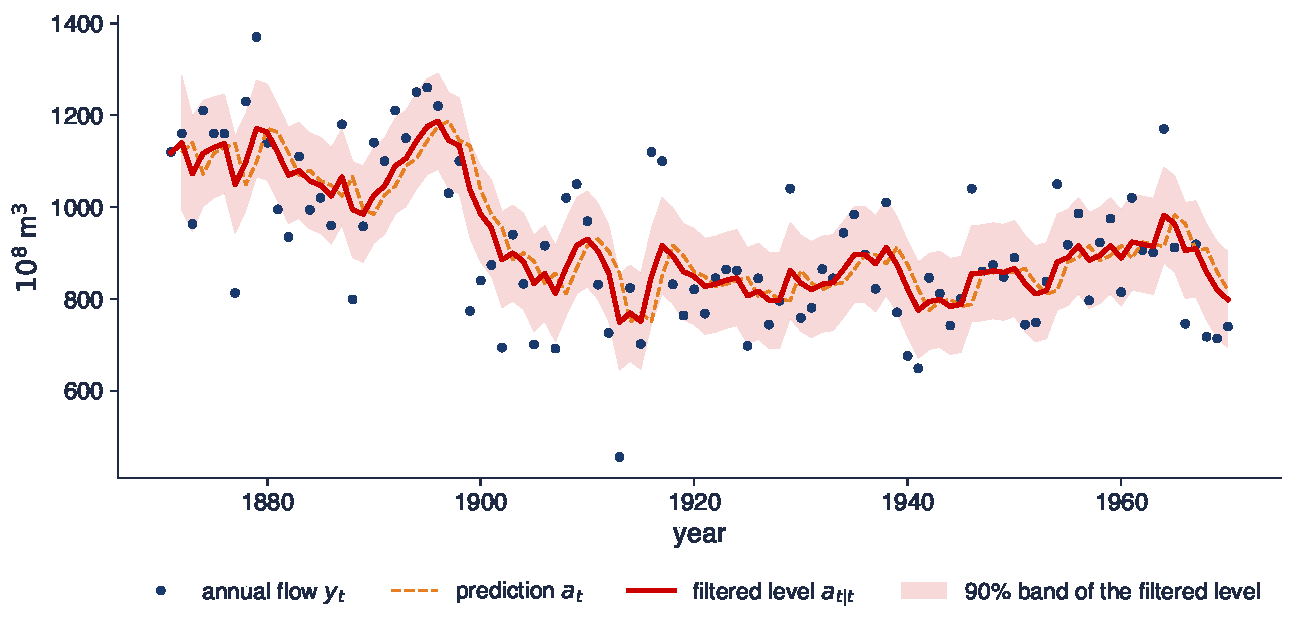
\includegraphics[width=0.97\textwidth,height=0.58\textheight,keepaspectratio]{tsa_ch10_nile_filter.pdf}
\end{center}
\vspace{-0.25cm}
\begin{itemize}
    \item Annual flow at Aswan, 1871--1970 ($10^8$ m$^3$, statsmodels); variances by maximum likelihood with a diffuse start: $\hat\sigma^2_\varepsilon = 15100$, $\hat\sigma^2_\eta = 1468$, $\hat q = 0.097$, the estimates of \refDK
\end{itemize}
\quantlet{TSA\_ch10\_kalman\_filter}{\qlurl{TSA_ch10_kalman_filter}}
\end{frame}

\begin{frame}{Interpreting the Nile filter}
\itemsize{\small}
\begin{itemize}
    \item Most of the year-to-year movement is noise: $\hat q = 0.097$, so each flow moves the level by about a quarter of the surprise ($\bar K = 0.267$)
    \begin{itemize}
        \item \texttt{statsmodels} \texttt{UnobservedComponents('llevel')} gives 15078 and 1479: the same model, a slightly different start
    \end{itemize}
    \item 1899: the flow is 774, the predicted level 1133; the surprise $v = \ensuremath{-}359$ lowers the level only to 1037
    \begin{itemize}
        \item the filter needs several low years to accept the new level (834 in 1905): the first Aswan dam was completed in 1902
    \end{itemize}
    \item In 1970 the level is 798 with standard error 63, well below the sample mean 919
\end{itemize}
\end{frame}

\begin{frame}{The gain converges; SES reproduces the filter}
\itemsize{\footnotesize}
\begin{center}
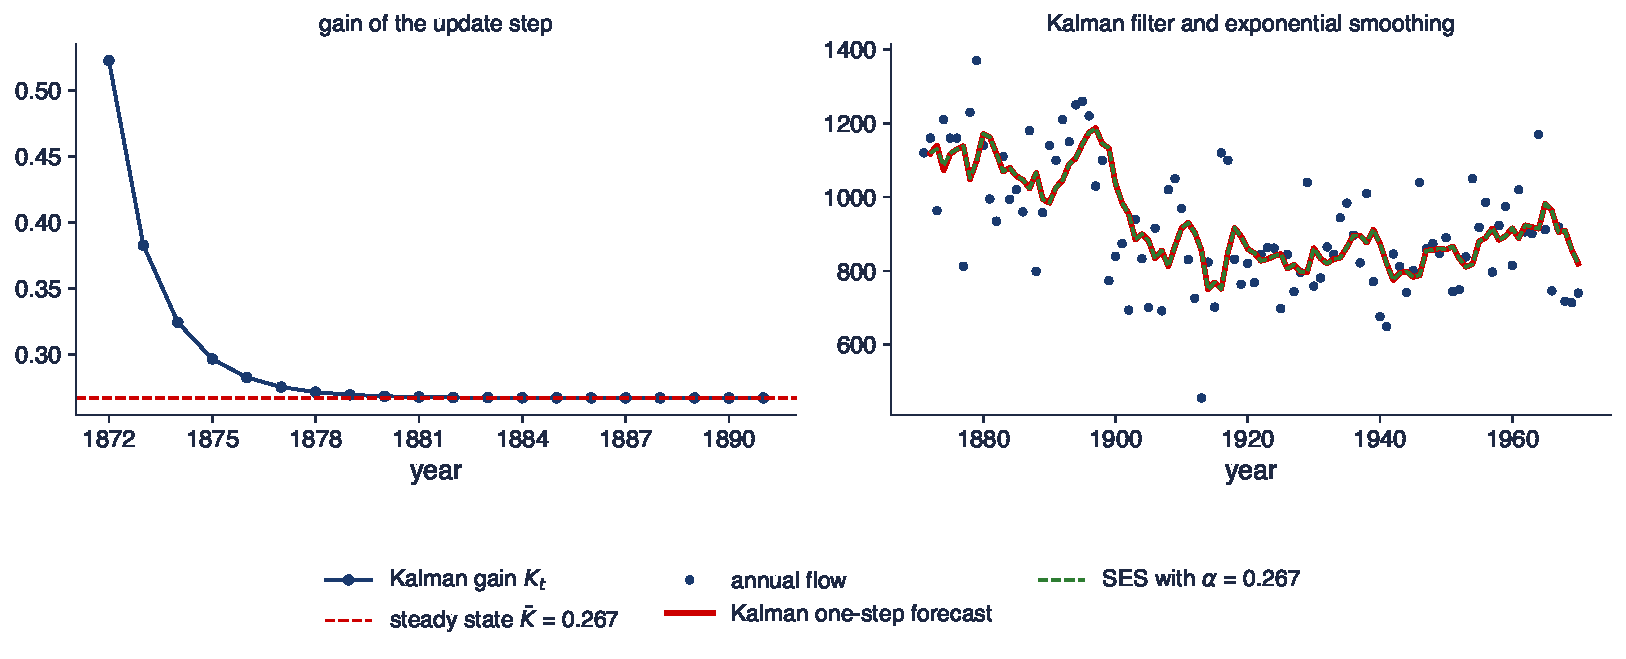
\includegraphics[width=0.97\textwidth,height=0.66\textheight,keepaspectratio]{tsa_ch10_gain_ses.pdf}
\end{center}
\vspace{-0.25cm}
\begin{itemize}
    \item Left: $K_t$ of the Nile filter; right: the Kalman one-step forecasts $a_{t}$ and SES with $\alpha = \bar K$, started at the first observation
\end{itemize}
\quantlet{TSA\_ch10\_kalman\_filter}{\qlurl{TSA_ch10_kalman_filter}}
\end{frame}

\begin{frame}{Interpreting the gain}
\itemsize{\small}
\begin{itemize}
    \item $K_t$ starts at 0.523 (after the diffuse start), 0.297 in year 5, and is within 0.001 of $\bar K = 0.267$ after 10 years
    \begin{itemize}
        \item the forecasts differ by 0.24 in year 5 and by less than 0.02 after 20 years
    \end{itemize}
    \item SES fitted directly by least squares (\tsachlink{https://danpele.github.io/Time-Series-Analysis/EN/Courses/chapter0_introduction.pdf}{Chapter 0}) gives $\hat\alpha = 0.246$, i.e.\ $q = \alpha^2/(1-\alpha) = 0.080$
    \begin{itemize}
        \item close to the likelihood answer: two criteria, one model
    \end{itemize}
    \item The state space view explains SES: $\alpha$ is large when the level moves a lot relative to the noise
\end{itemize}
\end{frame}

\begin{frame}{Recap: The Kalman filter}
\itemsize{\small}
\begin{itemize}
    \item Update: $v_t = y_t - Z_ta_t$, $F_t = Z_tP_tZ_t' + H$, $K_t = P_tZ_t'F_t^{-1}$, $a_{t|t} = a_t + K_tv_t$
    \item Prediction: $a_{t+1} = Ta_{t|t}$, $P_{t+1} = TP_{t|t}T' + RQR'$
    \item The gain weighs the data against the model; it settles at a steady state
    \item Local level in steady state = SES with $\alpha = \bar K$; Nile: $\bar K = 0.267$
\end{itemize}
\end{frame}


%=============================================================================
\section{Smoothing, likelihood and missing data}
%=============================================================================

\begin{frame}{Smoothing: using the whole sample}
\itemsize{\small}
\begin{itemize}
    \item \textbf{Filtering} uses $Y_t$ (the past and the present): the real-time estimate
    \begin{itemize}
        \item \textbf{smoothing} uses $Y_n$ (the whole sample): $\hat\alpha_t = E(\alpha_t \mid Y_n)$, with variance $V_t \le P_{t|t}$
    \end{itemize}
    \item \textbf{Rauch--Tung--Striebel} smoother \refRTS: one backward pass after the filter, from $t = n-1$ to 1
    \begin{itemize}
        \item $n$: the sample size; $J_t$: the smoother gain, the weight of the revision coming from the future
        \item $J_t = P_{t|t}T'P_{t+1}^{-1}$, \quad $\hat\alpha_t = a_{t|t} + J_t(\hat\alpha_{t+1} - a_{t+1})$
        \item $V_t = P_{t|t} + J_t(V_{t+1} - P_{t+1})J_t'$; at $t = n$ smoothed and filtered coincide
    \end{itemize}
    \item Use: the filtered state for decisions in real time and forecasting; the smoothed state for history (dating breaks, the past output gap)
\end{itemize}
\end{frame}

\begin{frame}{The Nile: filtered against smoothed level}
\itemsize{\footnotesize}
\begin{center}
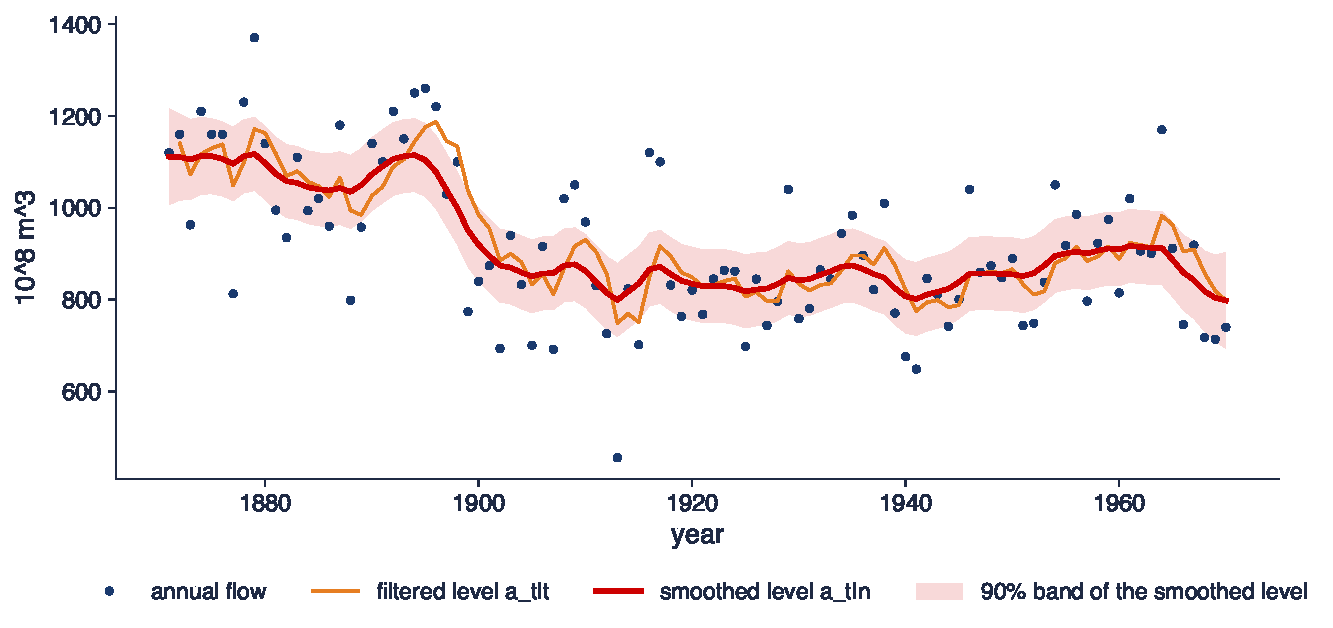
\includegraphics[width=0.97\textwidth,height=0.58\textheight,keepaspectratio]{tsa_ch10_nile_smooth.pdf}
\end{center}
\vspace{-0.25cm}
\begin{itemize}
    \item Filtered level $a_{t|t}$ and smoothed level $\hat\alpha_t$ with its 90\% band; the same maximum-likelihood variances
\end{itemize}
\quantlet{TSA\_ch10\_smoothing\_likelihood}{\qlurl{TSA_ch10_smoothing_likelihood}}
\end{frame}

\begin{frame}{Interpreting the smoothed level}
\itemsize{\small}
\begin{itemize}
    \item The smoothed level reacts to the 1898--1899 drop \textbf{before} it happens in the data: in 1897 it is already 1038, against 1145 filtered
    \begin{itemize}
        \item it knows the future: useful for history, impossible in real time
    \end{itemize}
    \item In 1900: smoothed 920, filtered 985; the smoothed level adapts faster because it sees the low years after 1900
    \begin{itemize}
        \item standard error in 1920: 48 smoothed against 63 filtered
    \end{itemize}
    \item The smoothed path shows a step near 1899 more clearly than any moving average of \tsachlink{https://danpele.github.io/Time-Series-Analysis/EN/Courses/chapter0_introduction.pdf}{Chapter 0}
\end{itemize}
\end{frame}

\begin{frame}{The likelihood: prediction-error decomposition}
\itemsize{\small}
\begin{itemize}
    \item The joint density factorises into one-step conditional densities: $p(y_1, \dots, y_n) = \prod_t p(y_t \mid Y_{t-1})$
    \begin{itemize}
        \item with Gaussian errors, $y_t \mid Y_{t-1} \sim N(Z_ta_t, F_t)$: the filter delivers the mean and the variance
    \end{itemize}
    \item \textbf{Prediction-error decomposition}
    \begin{itemize}
        \item $\log L(\theta) = -\dfrac{n}{2}\log 2\pi - \dfrac12\sum_{t=1}^{n}\left(\log F_t + \dfrac{v_t^2}{F_t}\right)$
        \item $\theta$: the parameters (the variances of the model); $v_t$, $F_t$: the prediction errors and their variances, from the filter
        \item one run of the filter gives $\log L$ for one value of $\theta$; a numerical optimiser searches over $\theta$
    \end{itemize}
    \item Diffuse start: the first $d$ terms (here $d = 1$ for the level) are left out, since $F_t$ is huge there \refDK
    \item The same idea as the exact ARMA likelihood of \tsachlink{https://danpele.github.io/Time-Series-Analysis/EN/Courses/chapter2_arma_models.pdf}{Chapter 2}, now for any state space model
\end{itemize}
\end{frame}

\begin{frame}{Maximum likelihood in practice}
\itemsize{\small}
\begin{itemize}
    \item Optimise over $\log\sigma^2$ (variances stay positive); several starting values, since the surface can be flat
    \begin{itemize}
        \item a variance estimated at zero is common and meaningful: that component is deterministic
    \end{itemize}
    \item \textbf{Concentrating}: for the local level, write $\sigma^2_\eta = q\sigma^2_\varepsilon$; for fixed $q$, $\hat\sigma^2_\varepsilon = \frac{1}{n-1}\sum_t v_t^2/F_t$ in closed form
    \begin{itemize}
        \item the profile log-likelihood is then a function of $q$ alone (next chart)
    \end{itemize}
    \item Standard errors from the numerical Hessian; model choice by AIC and BIC; tests on the standardised prediction errors $e_t = v_t/\sqrt{F_t}$
    \begin{itemize}
        \item \texttt{statsmodels}: \texttt{UnobservedComponents}, \texttt{SARIMAX}, \texttt{DynamicFactor} all use this machinery
    \end{itemize}
\end{itemize}
\end{frame}

\begin{frame}{Profile likelihood and the choice of $q$}
\itemsize{\footnotesize}
\begin{center}
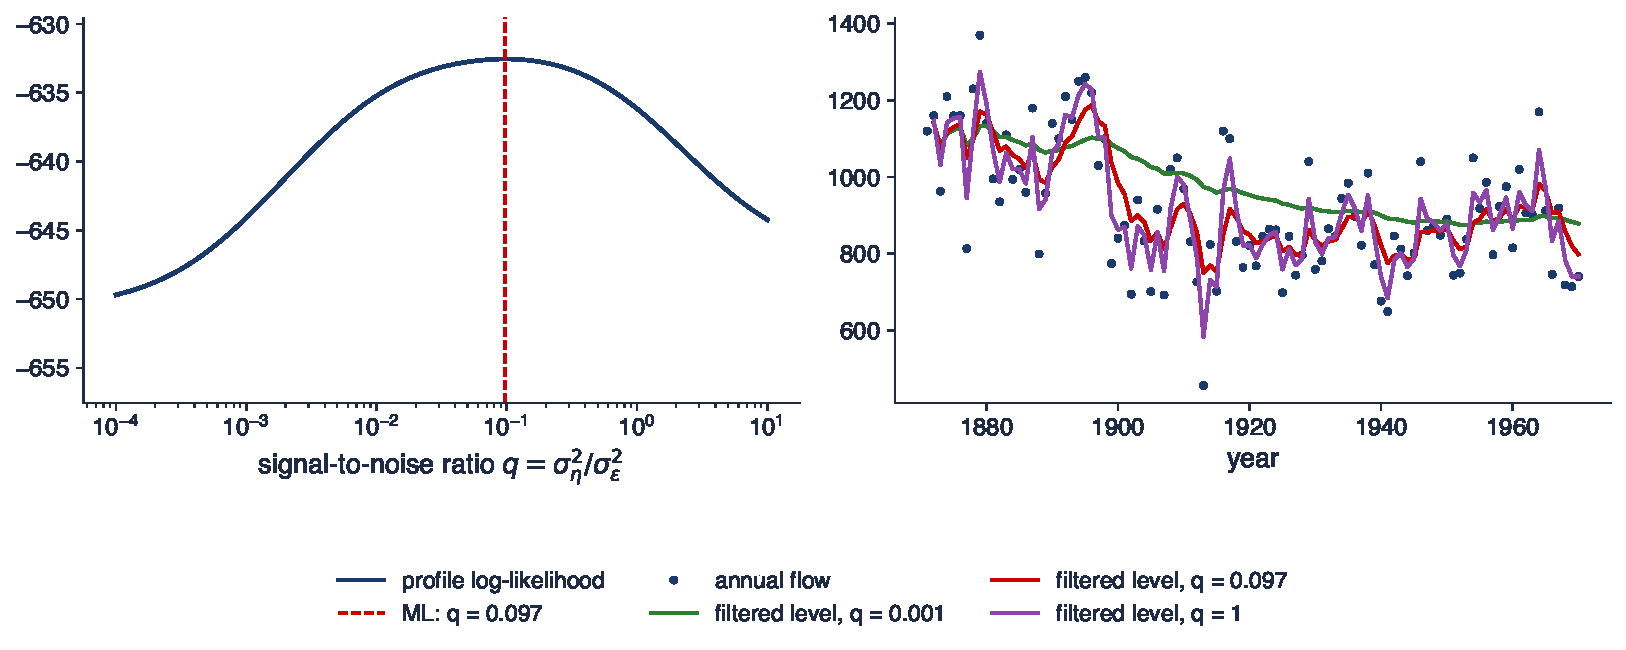
\includegraphics[width=0.97\textwidth,height=0.66\textheight,keepaspectratio]{tsa_ch10_likelihood.pdf}
\end{center}
\vspace{-0.25cm}
\begin{itemize}
    \item Left: profile log-likelihood of the Nile local level model against $q$ (log scale); right: filtered levels for $q = 0.001$, the ML value and $q = 1$
\end{itemize}
\quantlet{TSA\_ch10\_smoothing\_likelihood}{\qlurl{TSA_ch10_smoothing_likelihood}}
\end{frame}

\begin{frame}{Interpreting the profile likelihood}
\itemsize{\small}
\begin{itemize}
    \item A clear maximum at $\hat q = 0.097$, with $\hat\sigma^2_\varepsilon = 15100$ from the closed form
    \begin{itemize}
        \item likelihood-ratio statistic against $q = 0.001$ (an almost constant level): 23.1; against $q = 1$: 7.2
    \end{itemize}
    \item Small $q$: the level is almost flat and misses the drop after 1899; large $q$: the level chases every flood
    \begin{itemize}
        \item the likelihood picks the compromise that predicts best one step ahead
    \end{itemize}
    \item Choosing $q$ is the same as choosing the SES weight $\alpha$ in \tsachlink{https://danpele.github.io/Time-Series-Analysis/EN/Courses/chapter0_introduction.pdf}{Chapter 0}, now with a statistical criterion
\end{itemize}
\end{frame}

\begin{frame}{Diagnostics}
\itemsize{\small}
\begin{itemize}
    \item If the model is right, the standardised prediction errors $e_t = v_t/\sqrt{F_t}$ are i.i.d. $N(0, 1)$
    \begin{itemize}
        \item the checks of \tsachlink{https://danpele.github.io/Time-Series-Analysis/EN/Courses/chapter1_stochastic_processes_stationarity.pdf}{Chapters 1}--\tsachlink{https://danpele.github.io/Time-Series-Analysis/EN/Courses/chapter2_arma_models.pdf}{2}: the ACF and the Ljung--Box test (independence), Jarque--Bera (normality), a plot over time (outliers)
    \end{itemize}
    \item \textbf{Auxiliary residuals} \refDK: the smoothed disturbances $\hat\varepsilon_t$ and $\hat\eta_t$, standardised
    \begin{itemize}
        \item a large $\hat\varepsilon_t$: an \textbf{outlier} in one observation
        \item a large $\hat\eta_t$: a \textbf{break} in the level, a permanent shift
    \end{itemize}
    \item Computed by a backward recursion (the disturbance smoother) after the filter
\end{itemize}
\end{frame}

\begin{frame}{Diagnostics of the Nile model}
\itemsize{\footnotesize}
\begin{center}
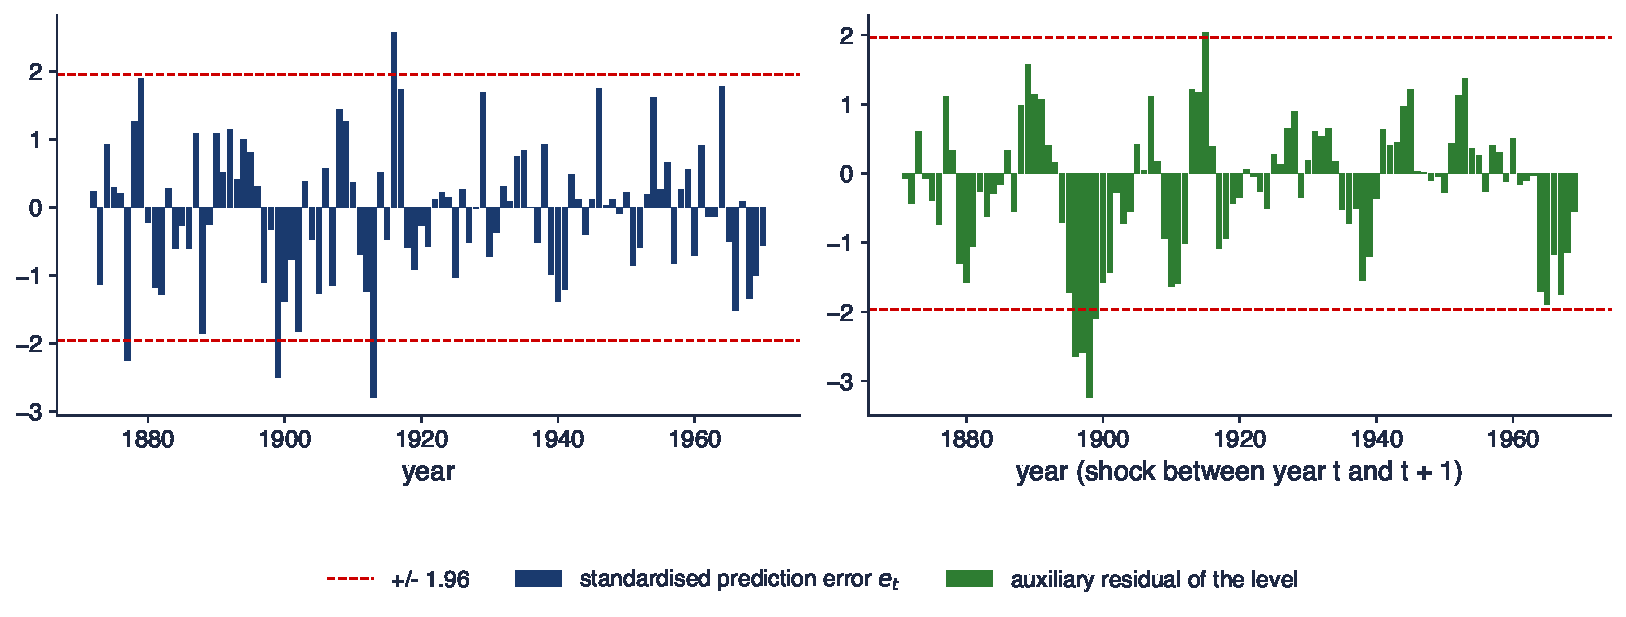
\includegraphics[width=0.97\textwidth,height=0.66\textheight,keepaspectratio]{tsa_ch10_diagnostics.pdf}
\end{center}
\vspace{-0.25cm}
\begin{itemize}
    \item Left: standardised one-step prediction errors $e_t$; right: standardised auxiliary residual of the level, $\hat\eta_t$ (a shock between year $t$ and $t+1$); dashed: $\pm 1.96$
\end{itemize}
\quantlet{TSA\_ch10\_smoothing\_likelihood}{\qlurl{TSA_ch10_smoothing_likelihood}}
\end{frame}

\begin{frame}{Interpreting the diagnostics}
\itemsize{\small}
\begin{itemize}
    \item Prediction errors: Ljung--Box $Q(10) = 13.2$ (p = 0.21), Jarque--Bera 0.05 (p = 0.98); 4 of 99 outside $\pm 1.96$
    \begin{itemize}
        \item no evidence against the model in the one-step errors
    \end{itemize}
    \item The level residual has its minimum in 1898 (\ensuremath{-}3.23): the shift of the level between 1898 and 1899
    \begin{itemize}
        \item the observation residual has its minimum in 1913 (\ensuremath{-}3.04): a single very dry year, an outlier
    \end{itemize}
    \item The same break as in \tsachlink{https://danpele.github.io/Time-Series-Analysis/EN/Courses/chapter8_long_memory_arfima.pdf}{Chapter 8} (spurious long memory of the Nile), now located by the model itself
\end{itemize}
\end{frame}

\begin{frame}{Missing values and forecasting}
\itemsize{\small}
\begin{itemize}
    \item A missing $y_t$: no update; $a_{t+1} = Ta_t$, $P_{t+1} = TP_tT' + RQR'$
    \begin{itemize}
        \item the likelihood simply skips that term; nothing is interpolated by hand
    \end{itemize}
    \item Forecasting $h$ steps ahead = treating $y_{n+1}, \dots, y_{n+h}$ as missing
    \begin{itemize}
        \item local level: $\hat y_{n+h} = a_{n+1}$ for every $h$, with variance $P_{n+1} + (h-1)\sigma^2_\eta + \sigma^2_\varepsilon$
    \end{itemize}
    \item Uses: irregular data (holidays), series that start at different dates, mixed frequencies, the ragged edge of a nowcast
    \begin{itemize}
        \item the smoother fills the gaps with $\hat\alpha_t$ and the corresponding standard error
    \end{itemize}
\end{itemize}
\end{frame}

\begin{frame}{Missing years and forecasts of the Nile}
\itemsize{\footnotesize}
\begin{center}
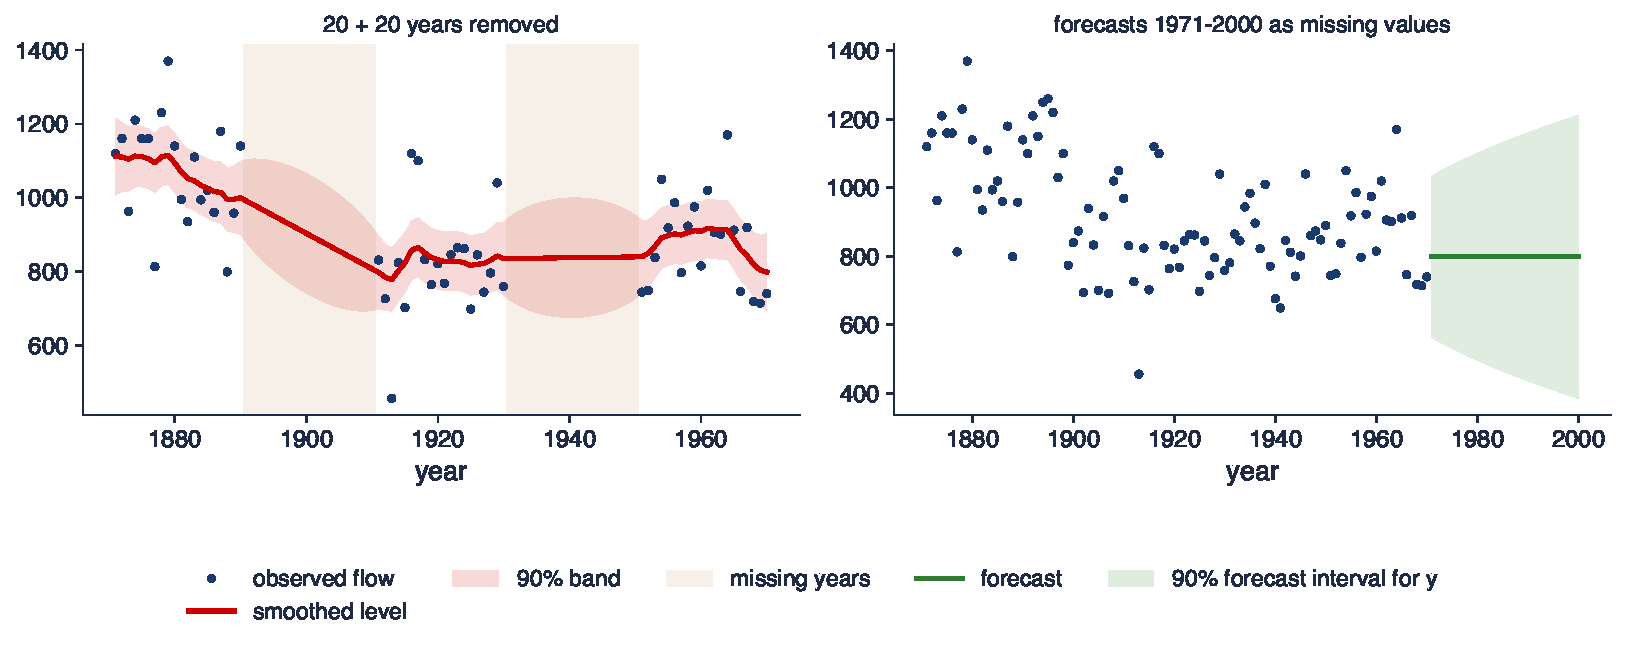
\includegraphics[width=0.97\textwidth,height=0.66\textheight,keepaspectratio]{tsa_ch10_missing.pdf}
\end{center}
\vspace{-0.25cm}
\begin{itemize}
    \item Left: 1891--1910 and 1931--1950 removed (the experiment of \refDK), smoothed level with 90\% band; right: forecasts for 1971--2000 with 90\% intervals for $y$
\end{itemize}
\quantlet{TSA\_ch10\_missing\_data}{\qlurl{TSA_ch10_missing_data}}
\end{frame}

\begin{frame}{Interpreting the missing data}
\itemsize{\small}
\begin{itemize}
    \item Inside a gap the smoothed level is a straight line between the two edges; its standard error grows to 99 in 1900, against 48 with all data
    \begin{itemize}
        \item the band widens towards the middle of the gap and narrows near observed years
    \end{itemize}
    \item Forecasts are flat at 798: a random-walk level has no predictable direction
    \begin{itemize}
        \item standard error of $y$: 144 one year ahead, 251 after 30 years
    \end{itemize}
    \item The same code handles missing data, forecasts and estimation: one of the main practical strengths of state space models
\end{itemize}
\end{frame}

\begin{frame}{Recap: Smoothing, likelihood and missing data}
\itemsize{\small}
\begin{itemize}
    \item Filtered: real time; smoothed (RTS): the whole sample, smaller variance
    \item $\log L = -\frac12\sum(\log 2\pi + \log F_t + v_t^2/F_t)$, maximised numerically
    \item Diagnostics on $e_t$; auxiliary residuals find outliers and breaks (Nile 1898--1899)
    \item Missing data and forecasts: skip the update step
\end{itemize}
\end{frame}


%=============================================================================
\section{Trend, cycle and common factors}
%=============================================================================

\begin{frame}{Unobserved components models}
\itemsize{\small}
\begin{itemize}
    \item \textbf{Structural time series} or \textbf{unobserved components} (UC) model \refHarvey: $y_t = \mu_t + \psi_t + \gamma_t + \varepsilon_t$
    \begin{itemize}
        \item trend $\mu_t$ (local level or local linear trend), cycle $\psi_t$, seasonal $\gamma_t$, irregular $\varepsilon_t$
        \item the decomposition of \tsachlink{https://danpele.github.io/Time-Series-Analysis/EN/Courses/chapter0_introduction.pdf}{Chapter 0}, but each component is a stochastic process with its own variance
    \end{itemize}
    \item The \textbf{cycle}: a stationary AR(2) $\psi_t = \phi_1\psi_{t-1} + \phi_2\psi_{t-2} + \kappa_t$, or a damped stochastic cycle with period $2\pi/\lambda_c$
    \begin{itemize}
        \item $\phi_1$, $\phi_2$: the AR coefficients of the cycle; $\kappa_t$: the cycle shock; $\lambda_c$: the frequency of the cycle, in radians
        \item for log GDP, $\psi_t$ is the \textbf{output gap}: the percentage deviation of output from its trend (potential)
    \end{itemize}
    \item In Python: \texttt{UnobservedComponents(y, level='smooth trend', autoregressive=2)}; the whole state is estimated by the Kalman filter and smoother
\end{itemize}
\end{frame}

\begin{frame}{The HP filter is a state space smoother}
\itemsize{\small}
\begin{itemize}
    \item \refHPf: the trend $\tau_t$ minimises $\sum_t(y_t - \tau_t)^2 + \lambda\sum_t(\Delta^2\tau_t)^2$; $\lambda = 1600$ for quarterly data
    \begin{itemize}
        \item $\Delta^2\tau_t = \tau_t - 2\tau_{t-1} + \tau_{t-2}$: the change in the slope of the trend; $\lambda \ge 0$: the smoothing parameter
        \item large $\lambda$: a straight-line trend; $\lambda = 0$: the trend is the series itself
    \end{itemize}
    \item This is exactly the \textbf{smoothed} trend of a UC model: smooth trend ($\Delta^2\mu_{t+1} = \zeta_t$) plus white noise, with $\lambda = \sigma^2_\varepsilon/\sigma^2_\zeta$ \refHJ
    \begin{itemize}
        \item the HP filter imposes the signal-to-noise ratio and a white-noise gap; the UC model estimates both
    \end{itemize}
    \item Being a smoother, HP uses future data: its last values are revised as new quarters arrive
\end{itemize}
\end{frame}

\begin{frame}{Hamilton (2018): why you should never use the HP filter}
\itemsize{\small}
\begin{itemize}
    \item \refHamHP\ lists three problems
    \begin{itemize}
        \item the HP gap of a random walk has cycles that are not in the data: spurious dynamics
        \item the end of the sample is treated differently from the middle: large revisions, misleading real-time gaps
        \item $\lambda = 1600$ is a convention, far from the value a likelihood would choose
    \end{itemize}
    \item His alternative, the \textbf{regression filter}: OLS of $y_{t+h}$ on $1, y_t, y_{t-1}, y_{t-2}, y_{t-3}$ with $h = 8$ quarters
    \begin{itemize}
        \item the cycle is the residual: what could not be predicted two years earlier; one-sided by construction
    \end{itemize}
    \item No method is the truth: we compare the UC model, HP and the Hamilton filter on Romanian GDP
\end{itemize}
\end{frame}

\begin{frame}{Romanian GDP: trend}
\itemsize{\footnotesize}
\begin{center}
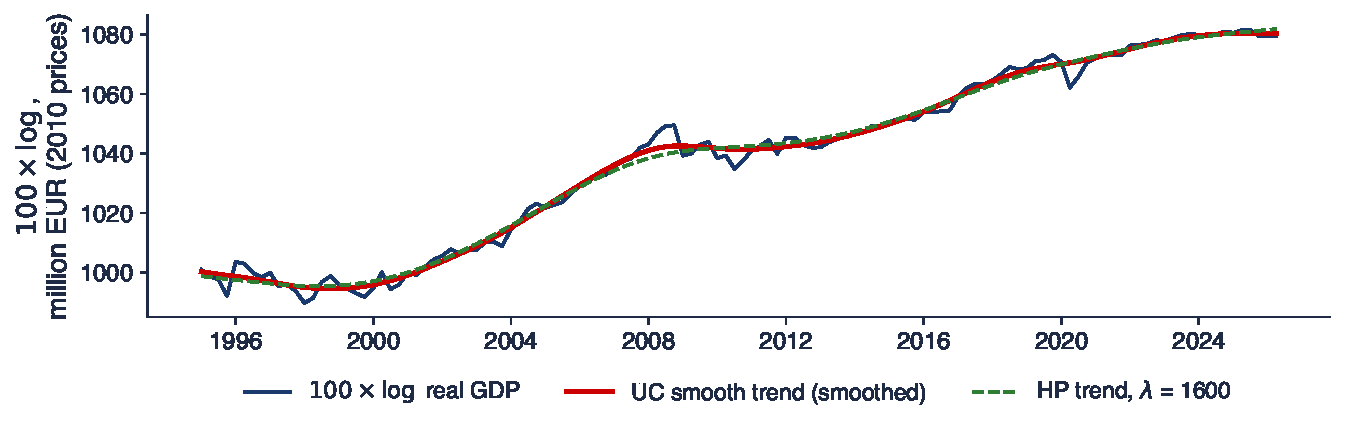
\includegraphics[width=0.97\textwidth,height=0.58\textheight,keepaspectratio]{tsa_ch10_ro_trend.pdf}
\end{center}
\vspace{-0.25cm}
\begin{itemize}
    \item $100 \times \log$ of real GDP, quarterly, seasonally and calendar adjusted, chain-linked volumes (Eurostat namq\_10\_gdp), 1995Q1--2026Q2 ($T = 126$); UC model: smooth trend plus AR(2) cycle; HP with $\lambda = 1600$
\end{itemize}
\quantlet{TSA\_ch10\_trend\_cycle}{\qlurl{TSA_ch10_trend_cycle}}
\end{frame}

\begin{frame}{Interpreting the trend}
\itemsize{\small}
\begin{itemize}
    \item Average growth 2.5\% per year, with a slow start (the 1997--1999 recession), a boom until 2008, a stagnation and a recovery after 2013
    \begin{itemize}
        \item the two trends are almost identical: the difference between methods lies in the gap, not in the trend
    \end{itemize}
    \item UC estimates: $\hat\sigma^2_\zeta = 0.078$ (trend slope), cycle AR(2) with $\hat\phi_1 = 0.61$, $\hat\phi_2 = \ensuremath{-}0.13$, $\hat\sigma^2_\kappa = 5.27$; the irregular variance is estimated at zero
    \begin{itemize}
        \item the ratio cycle variance / trend variance is 68, far below the 1600 that HP imposes: a more flexible trend
    \end{itemize}
    \item A flexible trend absorbs part of the boom: the UC gap will be smaller than the HP gap
\end{itemize}
\end{frame}

\begin{frame}{The Romanian output gap: three methods}
\itemsize{\footnotesize}
\begin{center}
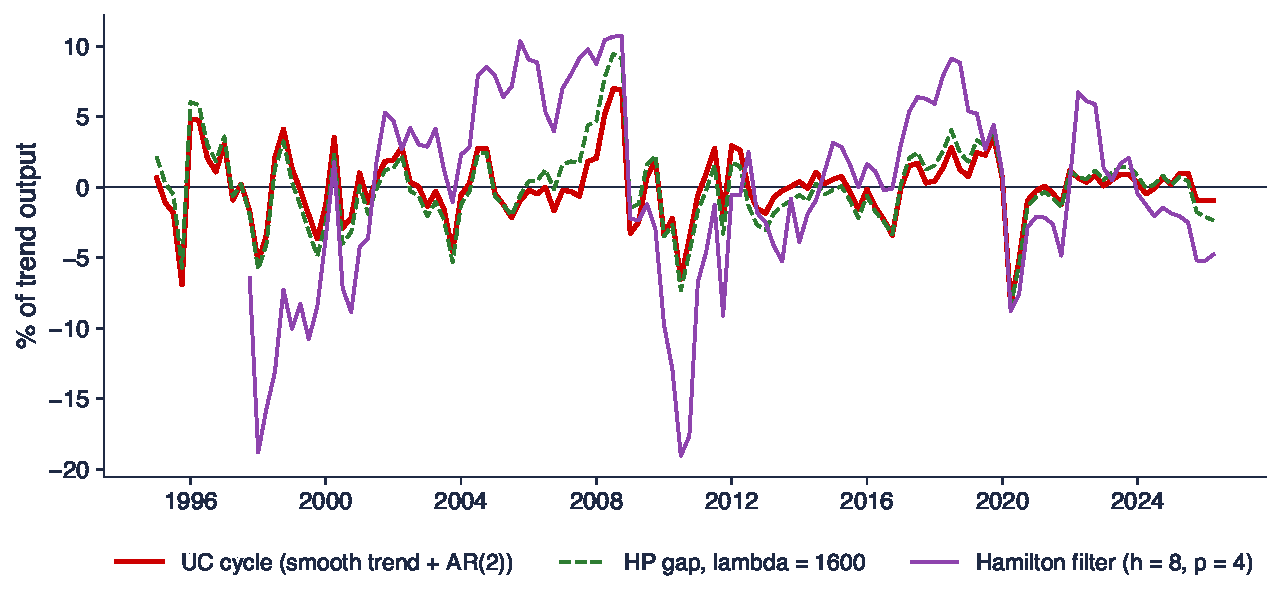
\includegraphics[width=0.97\textwidth,height=0.58\textheight,keepaspectratio]{tsa_ch10_output_gap.pdf}
\end{center}
\vspace{-0.25cm}
\begin{itemize}
    \item Gap in \% of trend: UC cycle (smoothed), HP gap ($\lambda = 1600$) and the Hamilton filter ($h = 8$, four lags), the first 11 quarters lost
\end{itemize}
\quantlet{TSA\_ch10\_trend\_cycle}{\qlurl{TSA_ch10_trend_cycle}}
\end{frame}

\begin{frame}{Interpreting the output gaps}
\itemsize{\small}
\begin{itemize}
    \item All three see the overheating before 2008 (peaks: UC 7.0\% in 2008Q3, HP 9.5\%, Hamilton 10.7\%) and the 2020 pandemic (UC \ensuremath{-}8.3\%, HP \ensuremath{-}8.5\%)
    \begin{itemize}
        \item correlations: UC--HP 0.94, UC--Hamilton 0.57, HP--Hamilton 0.69
    \end{itemize}
    \item Standard deviations: UC 2.4, HP 2.9, Hamilton 6.5: the Hamilton gap also contains every surprise of two years
    \begin{itemize}
        \item the four regression coefficients sum to 0.97: GDP is close to a random walk with drift
    \end{itemize}
    \item Latest gap (2026Q2): UC \ensuremath{-}0.9\%, HP \ensuremath{-}2.4\%, Hamilton \ensuremath{-}4.8\%: the sign agrees, the size does not
\end{itemize}
\end{frame}

\begin{frame}{Real time against hindsight}
\itemsize{\footnotesize}
\begin{center}
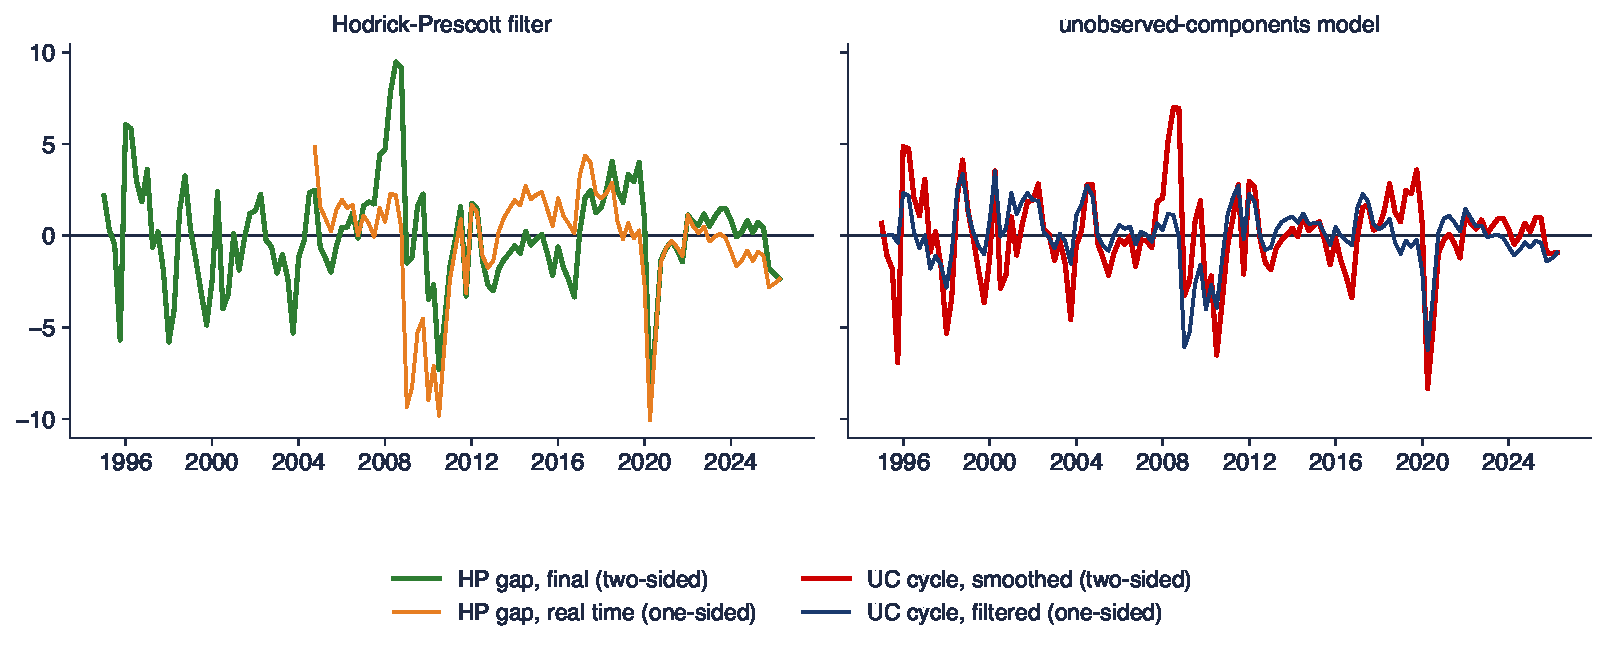
\includegraphics[width=0.97\textwidth,height=0.66\textheight,keepaspectratio]{tsa_ch10_realtime.pdf}
\end{center}
\vspace{-0.25cm}
\begin{itemize}
    \item Left: the HP gap computed with all data (two-sided) and the last value of the HP gap computed with the data available at each date (one-sided, from 2004); right: the UC cycle, filtered and smoothed
\end{itemize}
\quantlet{TSA\_ch10\_trend\_cycle}{\qlurl{TSA_ch10_trend_cycle}}
\end{frame}

\begin{frame}{Interpreting the revisions}
\itemsize{\small}
\begin{itemize}
    \item In 2008Q3 the real-time HP gap was 2.2\%; with hindsight it is 9.5\%: the overheating was invisible in real time
    \begin{itemize}
        \item the UC model shows the same problem: filtered 1.1\%, smoothed 7.0\%
    \end{itemize}
    \item Root mean square revision since 2004: HP 2.8 points, UC 1.8 points; correlation real time--final: HP 0.57, UC 0.65
    \begin{itemize}
        \item the end-point problem of \refHamHP; the UC model at least reports its own uncertainty
    \end{itemize}
    \item For policy in real time, use the filtered (one-sided) estimate and its standard error, never the last point of a two-sided filter
\end{itemize}
\end{frame}

\begin{frame}{A time-varying beta: the BET and the euro area}
\itemsize{\footnotesize}
\begin{center}
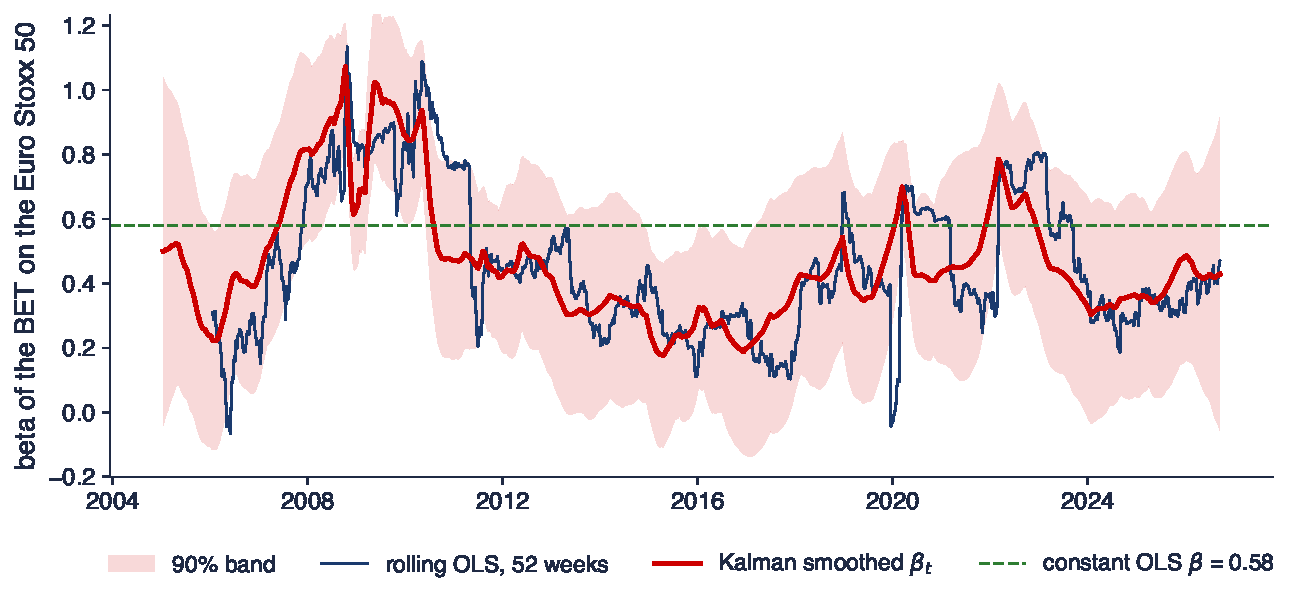
\includegraphics[width=0.97\textwidth,height=0.55\textheight,keepaspectratio]{tsa_ch10_tvp_beta.pdf}
\end{center}
\vspace{-0.25cm}
\begin{itemize}
    \item Weekly log returns of the BET on the Euro Stoxx 50 (EODHD), 2005--2026 ($T = 1\,126$ weeks)
    \item Random-walk beta by maximum likelihood, Kalman smoothed, with a 90\% band; 52-week rolling OLS; constant OLS
\end{itemize}
\quantlet{TSA\_ch10\_tvp\_regression}{\qlurl{TSA_ch10_tvp_regression}}
\end{frame}

\begin{frame}{Interpreting the time-varying beta}
\itemsize{\small}
\begin{itemize}
    \item The constant OLS beta is 0.58; the smoothed beta peaks at 1.07 (October 2008) and falls to 0.17 (April 2015)
    \begin{itemize}
        \item in the 2008 crisis the Romanian market moved almost one for one with the euro area; later it decoupled
    \end{itemize}
    \item Likelihood ratio against a constant beta: 46.1 (one restriction, a variance on the boundary): strong evidence of variation
    \begin{itemize}
        \item weekly standard deviation of the beta shocks 0.059; latest beta 0.43 with standard error 0.29
    \end{itemize}
    \item The rolling window jumps when a single extreme week enters or leaves it; the Kalman beta moves only as much as the likelihood allows
\end{itemize}
\end{frame}

\begin{frame}{Dynamic factor models and nowcasting}
\itemsize{\small}
\begin{itemize}
    \item \textbf{Dynamic factor model}: $y_{it} = \lambda_if_t + u_{it}$, \quad $f_t = \phi_1f_{t-1} + \phi_2f_{t-2} + \eta_t$
    \begin{itemize}
        \item many series $y_{1t}, \dots, y_{Nt}$ driven by one unobserved common factor $f_t$ (the state) with loadings $\lambda_i$
        \item $u_{it}$: the part of series $i$ not explained by the factor; $\phi_1$, $\phi_2$: the AR coefficients of the factor
        \item \refSW: a coincident index of US activity from four monthly indicators
    \end{itemize}
    \item \textbf{Nowcasting} \refGRS: estimate the current quarter before GDP is published
    \begin{itemize}
        \item monthly data arrive at different dates: the latest months of some series are missing (the \textbf{ragged edge})
        \item the Kalman filter treats them as missing values and updates the factor with whatever has arrived
    \end{itemize}
    \item Central banks use such models to nowcast GDP; \texttt{statsmodels} has \texttt{DynamicFactor} and \texttt{DynamicFactorMQ}
\end{itemize}
\end{frame}

\begin{frame}{A common factor of US activity}
\itemsize{\footnotesize}
\begin{center}
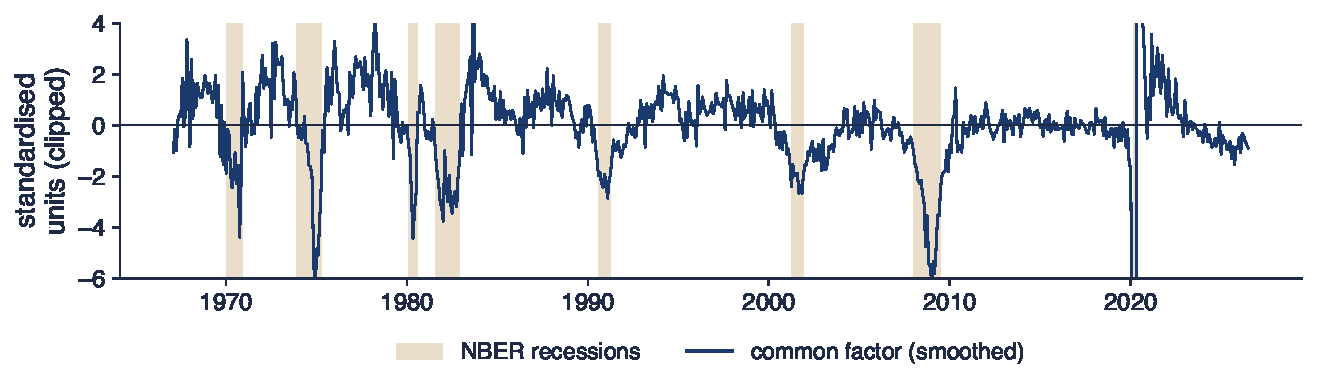
\includegraphics[width=0.97\textwidth,height=0.52\textheight,keepaspectratio]{tsa_ch10_dfm.pdf}
\end{center}
\vspace{-0.25cm}
\begin{itemize}
    \item Monthly growth of industrial production, payroll employment, real income less transfers and real manufacturing and trade sales (FRED), standardised
    \item One AR(2) factor estimated on 1967--2019 and run to July 2026; the last two months of income and sales set to missing
\end{itemize}
\quantlet{TSA\_ch10\_dynamic\_factor}{\qlurl{TSA_ch10_dynamic_factor}}
\end{frame}

\begin{frame}{Interpreting the common factor}
\itemsize{\small}
\begin{itemize}
    \item Loadings: employment 0.59, industrial production 0.42, sales 0.29, income 0.23; factor AR(2) with $\hat\phi_1 = 0.42$, $\hat\phi_2 = 0.41$
    \begin{itemize}
        \item correlation with the simple average of the four series: 0.86
    \end{itemize}
    \item Mean of the factor: \ensuremath{-}3.5 in NBER recession months, 0.4 in expansions; negative in 99\% of recession months
    \begin{itemize}
        \item April 2020: \ensuremath{-}74 standard units, off the scale of the chart
    \end{itemize}
    \item Latest value (July 2026): \ensuremath{-}0.9, computed although two of the four series are not yet available
\end{itemize}
\end{frame}

\begin{frame}{Recap: Trend, cycle and common factors}
\itemsize{\small}
\begin{itemize}
    \item UC models: trend + cycle + seasonal + irregular, each with its own variance
    \item HP = smoother of a UC model with imposed $\lambda$; Hamilton (2018): spurious cycles and end-point revisions
    \item Romanian output gap: the methods agree on the sign, not on the size; real-time gaps are revised heavily
    \item TVP regression and dynamic factors are state space models too
\end{itemize}
\end{frame}


%=============================================================================
\section{Markov switching}
%=============================================================================

\begin{frame}{Hamilton (1989) and the dating of recessions}
\itemsize{\footnotesize}
\begin{columns}[T]
\begin{column}{0.4\textwidth}
\centering
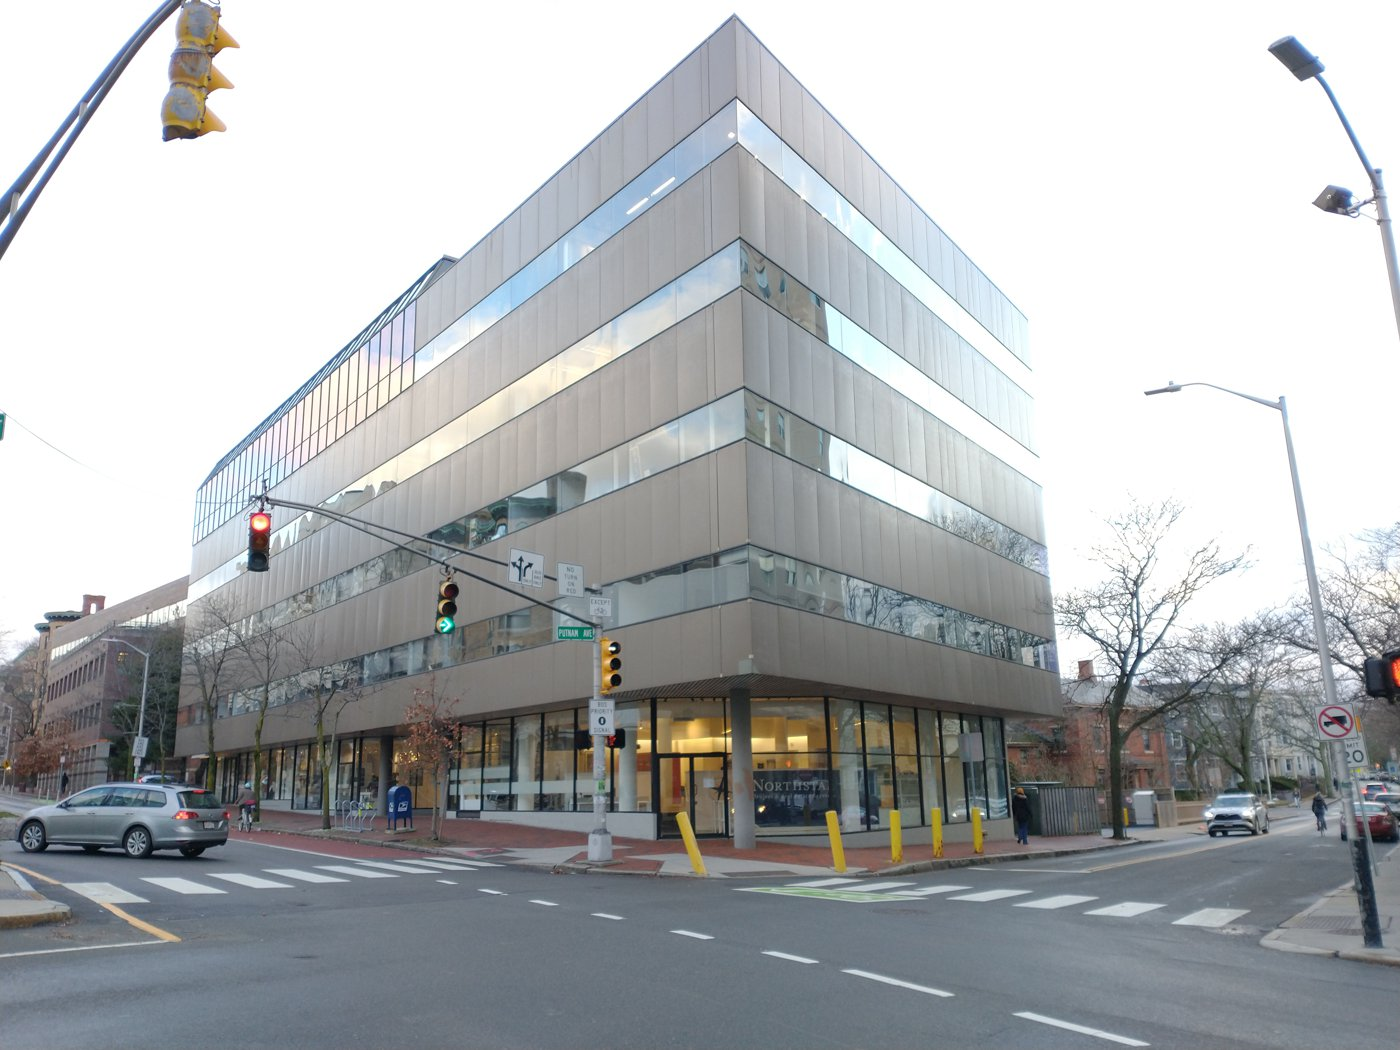
\includegraphics[height=0.36\textheight]{ch10_nber_offices_2022.jpg}\\[1mm]
\imgcap{The NBER, Cambridge (Massachusetts), whose committee dates US recessions}
\imgcredit{https://commons.wikimedia.org/wiki/File:National_Bureau_of_Economic_Research_offices.jpg}{Photo: Astrophobe (2022); CC BY-SA 4.0; Wikimedia Commons}
\end{column}
\begin{column}{0.58\textwidth}
\begin{itemize}
    \item The National Bureau of Economic Research (NBER) dates US recessions by a committee, months after the fact
    \begin{itemize}
        \item a recession is a regime: GDP behaves differently while it lasts
    \end{itemize}
    \item \refHamMS: let the mean of GDP growth depend on an unobserved regime $S_t \in \{1, 2\}$ that follows a Markov chain
    \begin{itemize}
        \item the data then tell us the probability of a recession in each quarter, without a committee
    \end{itemize}
    \item The state is now \textbf{discrete}; the Kalman filter is replaced by the Hamilton filter
\end{itemize}
\end{column}
\end{columns}
\end{frame}

\begin{frame}{The Markov-switching model}
\itemsize{\small}
\begin{itemize}
    \item \textbf{Switching mean}: $y_t = \mu_{S_t} + \varepsilon_t$, \quad $\varepsilon_t \sim N(0, \sigma^2_{S_t})$, \quad $S_t \in \{1, \dots, k\}$
    \begin{itemize}
        \item \textbf{Markov chain}: $p_{ij} = \Pr(S_t = j \mid S_{t-1} = i)$, constant over time; the rows of the transition matrix sum to 1
    \end{itemize}
    \item Hamilton's MS-AR(4): $y_t - \mu_{S_t} = \sum_{j=1}^{4}\phi_j(y_{t-j} - \mu_{S_{t-j}}) + \varepsilon_t$
    \begin{itemize}
        \item the AR dynamics stay the same; only the mean switches
    \end{itemize}
    \item Variants: switching variance (calm and turbulent markets), switching AR coefficients, $k = 3$ regimes
    \begin{itemize}
        \item in Python: \texttt{MarkovRegression}, \texttt{MarkovAutoregression} (\texttt{statsmodels})
    \end{itemize}
    \item A nonlinear model: the forecast depends on the probability of each regime
\end{itemize}
\end{frame}

\begin{frame}{Transition matrix, durations and ergodic probabilities}
\itemsize{\small}
\begin{itemize}
    \item Two regimes: $\mathbf{P} = \begin{pmatrix}p_{11} & 1 - p_{11}\\ 1 - p_{22} & p_{22}\end{pmatrix}$
    \begin{itemize}
        \item $h$-step transitions: $\mathbf{P}^h$
    \end{itemize}
    \item \textbf{Expected duration} of regime $i$: the time spent there is geometric, $\Pr(D = d) = p_{ii}^{d-1}(1 - p_{ii})$, so $E(D) = 1/(1 - p_{ii})$
    \begin{itemize}
        \item $p_{11} = 0.75$: recessions last $1/0.25 = 4$ quarters on average; $p_{22} = 0.95$: expansions last 20 quarters
    \end{itemize}
    \item \textbf{Ergodic} (long-run) probabilities: $\pi_1 = \dfrac{1 - p_{22}}{2 - p_{11} - p_{22}}$, the share of time spent in regime 1
    \begin{itemize}
        \item example: $\pi_1 = 0.05/0.30 = 1/6$: one quarter in six is a recession quarter
    \end{itemize}
\end{itemize}
\end{frame}

\begin{frame}{The Hamilton filter}
\itemsize{\small}
\begin{itemize}
    \item Track $\xi_{t|t} = \Pr(S_t = j \mid Y_t)$, the \textbf{filtered probabilities}, for each regime $j$
    \begin{itemize}
        \item \textbf{prediction}: $\Pr(S_t = j \mid Y_{t-1}) = \sum_i p_{ij}\Pr(S_{t-1} = i \mid Y_{t-1})$
        \item \textbf{densities}: $f_j(y_t) = \varphi\bigl((y_t - \mu_j)/\sigma_j\bigr)/\sigma_j$, the likelihood of $y_t$ in each regime
        \item $\varphi$: the standard Normal density; $\mu_j$, $\sigma_j$: the mean and standard deviation of regime $j$
        \item \textbf{update} (Bayes): $\Pr(S_t = j \mid Y_t) = \dfrac{\Pr(S_t = j \mid Y_{t-1})\,f_j(y_t)}{\sum_i\Pr(S_t = i \mid Y_{t-1})\,f_i(y_t)}$
    \end{itemize}
    \item The denominator is $p(y_t \mid Y_{t-1})$: the log-likelihood is $\sum_t\log p(y_t \mid Y_{t-1})$, as for the Kalman filter
    \begin{itemize}
        \item the same predict--update cycle, with probabilities instead of means and variances
    \end{itemize}
    \item Start: the ergodic probabilities $\pi_j$
\end{itemize}
\end{frame}

\begin{frame}{Smoothed probabilities and estimation}
\itemsize{\small}
\begin{itemize}
    \item \textbf{Smoothed probabilities} $\Pr(S_t = j \mid Y_n)$: a backward pass \refKim, the analogue of the RTS smoother
    \begin{itemize}
        \item used to date regimes in history; the filtered probabilities are what a forecaster knew at time $t$
    \end{itemize}
    \item Estimation: maximum likelihood by numerical optimisation, or the EM algorithm \refHamEM
    \begin{itemize}
        \item EM: expectation (smoothed probabilities given $\theta$) and maximisation (weighted means, variances, transition counts), repeated
    \end{itemize}
    \item The likelihood has \textbf{several local maxima}: use many random starting values and compare the solutions
    \begin{itemize}
        \item label switching: regime 1 and regime 2 can swap; name them by their means or variances
    \end{itemize}
\end{itemize}
\end{frame}

\begin{frame}{Hamilton's specification on today's data}
\itemsize{\small}
\begin{center}
\footnotesize
\begin{tabular}{>{\raggedright\arraybackslash}p{5.6cm}cc}
\toprule
\textbf{MS-AR(4), US real GDP growth, 1951Q2--1984Q4} & \textbf{Maximum A} & \textbf{Maximum B} \\
\midrule
mean, regime 1 / regime 2 (\% per quarter) & \ensuremath{-}0.14 / 1.32 & \ensuremath{-}1.14 / 0.96 \\
$p_{11}$, $p_{22}$ & 0.762, 0.892 & 0.128, 0.952 \\
expected duration, regime 1 / 2 (quarters) & 4.2 / 9.3 & 1.1 / 20.8 \\
log-likelihood & \ensuremath{-}189.47 & \ensuremath{-}189.16 \\
NBER recession quarters found (smoothed prob. $> 0.5$) & 94\% & 10\% \\
\bottomrule
\end{tabular}
\end{center}
\begin{itemize}
    \item Maximum A is Hamilton's answer: a recession regime of about four quarters that matches the NBER dates
    \item Maximum B has a slightly higher likelihood but a different meaning: isolated sharp quarters
    \item A likelihood difference of \ensuremath{-}189.16 against \ensuremath{-}189.47 cannot decide; economic meaning and robustness checks must
\end{itemize}
\end{frame}

\begin{frame}{US recessions from GDP growth}
\itemsize{\footnotesize}
\begin{center}
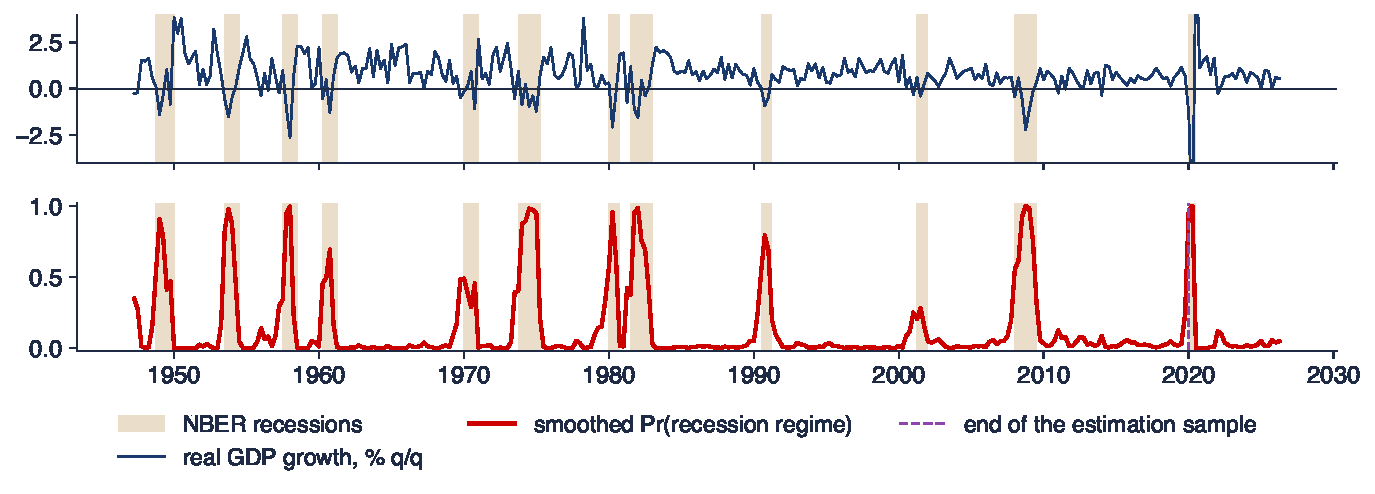
\includegraphics[width=0.97\textwidth,height=0.66\textheight,keepaspectratio]{tsa_ch10_ms_us.pdf}
\end{center}
\vspace{-0.25cm}
\begin{itemize}
    \item Two regimes with switching mean, constant variance, estimated on 48 NBER recession quarters out of 1947Q2--2019Q4 (FRED GDPC1, USREC); probabilities after 2019 computed with the same parameters
\end{itemize}
\quantlet{TSA\_ch10\_markov\_gdp}{\qlurl{TSA_ch10_markov_gdp}}
\end{frame}

\begin{frame}{Interpreting the recession probabilities}
\itemsize{\small}
\begin{itemize}
    \item Regime means: \ensuremath{-}0.42\% (recession) and 0.97\% (expansion) per quarter, $\hat\sigma = 0.79$; $\hat p_{11} = 0.685$, $\hat p_{22} = 0.949$
    \begin{itemize}
        \item expected durations: 3.2 quarters of recession, 19.7 quarters of expansion; ergodic share of recession 14\%
    \end{itemize}
    \item Agreement with the NBER: 94\% of quarters; 62\% of NBER recession quarters detected, 0\% false alarms
    \begin{itemize}
        \item the model misses the mild recessions (2001) and catches the deep ones
    \end{itemize}
    \item 2020Q2 ($\ensuremath{-}8.2\%$): probability 1.00, then back to expansion; after 2021 the probability never exceeds 0.12
\end{itemize}
\end{frame}

\begin{frame}{Filtered against smoothed probabilities: 2008}
\itemsize{\footnotesize}
\begin{center}
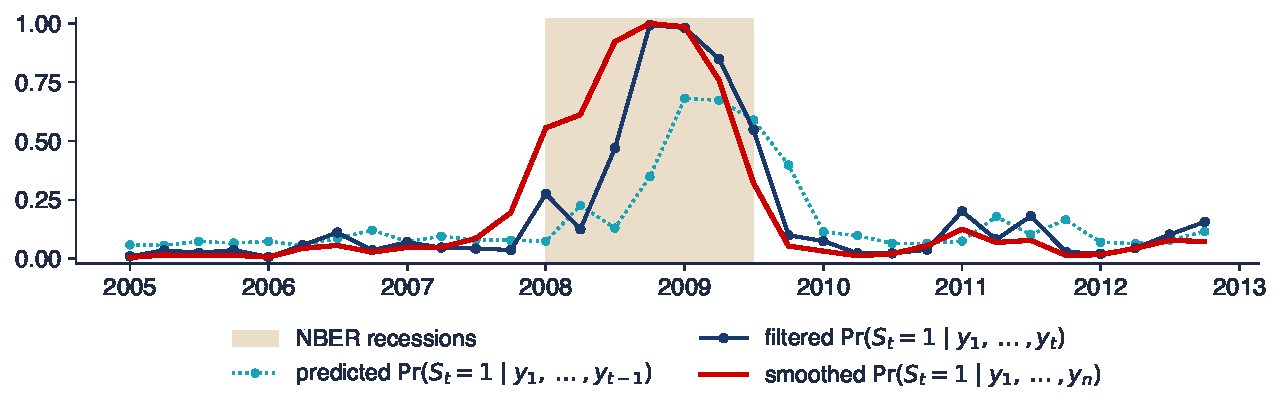
\includegraphics[width=0.97\textwidth,height=0.56\textheight,keepaspectratio]{tsa_ch10_ms_filtered.pdf}
\end{center}
\vspace{-0.25cm}
\begin{itemize}
    \item Predicted, filtered and smoothed probability of the recession regime, 2005--2012, same model as on the previous chart
\end{itemize}
\quantlet{TSA\_ch10\_markov\_gdp}{\qlurl{TSA_ch10_markov_gdp}}
\end{frame}

\begin{frame}{Interpreting the real-time probabilities}
\itemsize{\small}
\begin{itemize}
    \item The NBER recession started in 2008Q1; the smoothed probability crosses 0.5 in 2008Q1, the filtered one only in 2008Q4
    \begin{itemize}
        \item 2008Q1: filtered 0.28, smoothed 0.56; 2008Q3 (growth \ensuremath{-}0.53\%): filtered 0.47, smoothed 0.92
    \end{itemize}
    \item Concordance with the NBER using only filtered probabilities: 92\% of quarters, 54\% of recession quarters
    \begin{itemize}
        \item real-time dating is harder: \refCP\ compare the methods on real-time data
    \end{itemize}
    \item Never judge a model's real-time skill from its smoothed probabilities: they use the future
\end{itemize}
\end{frame}

\begin{frame}{Checks: which regimes did the model find?}
\itemsize{\small}
\begin{itemize}
    \item \textbf{Switching variance} on 1947--2019: the regimes become high and low volatility, not recession and expansion
    \begin{itemize}
        \item standard deviations 1.20 and 0.44; durations 45 and 39 quarters; the switch to the calm regime in 1984Q3
        \item this is the ``Great Moderation'' of the mid-1980s; agreement with the NBER falls to 60\% (47\% false alarms)
    \end{itemize}
    \item \textbf{Including 2020} in the estimation: one regime is the single quarter 2020Q2 (mean \ensuremath{-}8.2\%), the other lasts 315 quarters
    \begin{itemize}
        \item one extreme observation can capture a whole regime
    \end{itemize}
    \item Checklist: plot the probabilities against known events; compare several starting values and samples; prefer the specification with a clear economic meaning
\end{itemize}
\end{frame}

\begin{frame}{Romanian GDP growth regimes}
\itemsize{\footnotesize}
\begin{center}
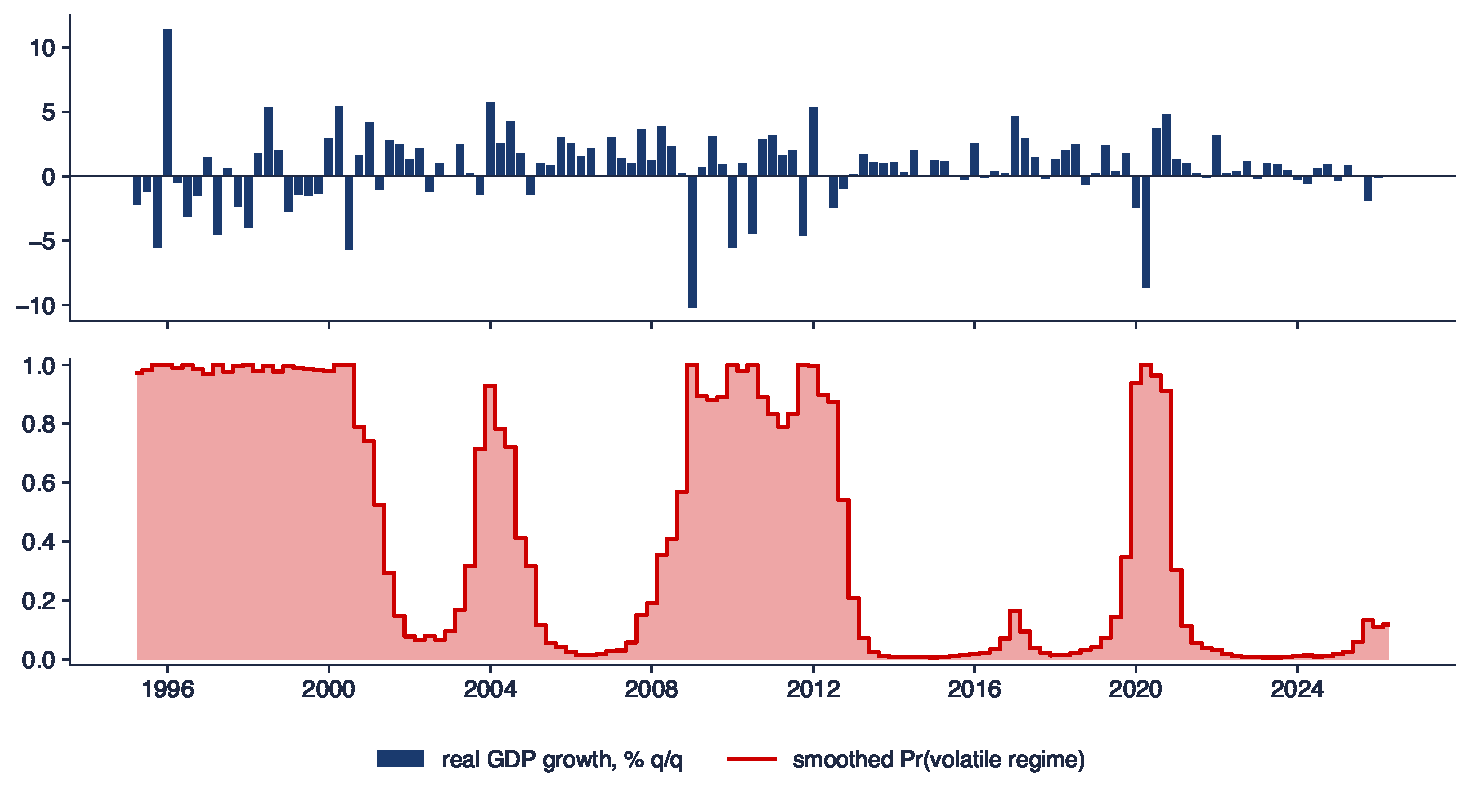
\includegraphics[width=0.97\textwidth,height=0.66\textheight,keepaspectratio]{tsa_ch10_ms_ro.pdf}
\end{center}
\vspace{-0.25cm}
\begin{itemize}
    \item Quarter-on-quarter growth of Romanian real GDP (Eurostat), two regimes with switching mean and variance; smoothed probability of the volatile regime
\end{itemize}
\quantlet{TSA\_ch10\_markov\_gdp}{\qlurl{TSA_ch10_markov_gdp}}
\end{frame}

\begin{frame}{Interpreting the Romanian regimes}
\itemsize{\small}
\begin{itemize}
    \item Stable regime: mean 1.03\% per quarter, standard deviation 1.3; volatile regime: mean 0.07\%, standard deviation 3.9
    \begin{itemize}
        \item expected durations: 15.2 quarters stable, 11.2 quarters volatile; 40\% of the quarters are volatile
    \end{itemize}
    \item Volatile spells: 1995Q2--2001Q2 (transition and the 1997--1999 recession), 2003Q4--2004Q3, 2008Q4--2012Q4 (the crisis and the austerity of 2010), 2020Q1--2020Q4 (the pandemic)
    \begin{itemize}
        \item latest probability of the volatile regime: 0.12
    \end{itemize}
    \item With 125 quarters a mean-only model is unstable; regimes of volatility and growth come together in an emerging economy
\end{itemize}
\end{frame}

\begin{frame}{Calm and turbulent stock markets}
\itemsize{\footnotesize}
\begin{center}
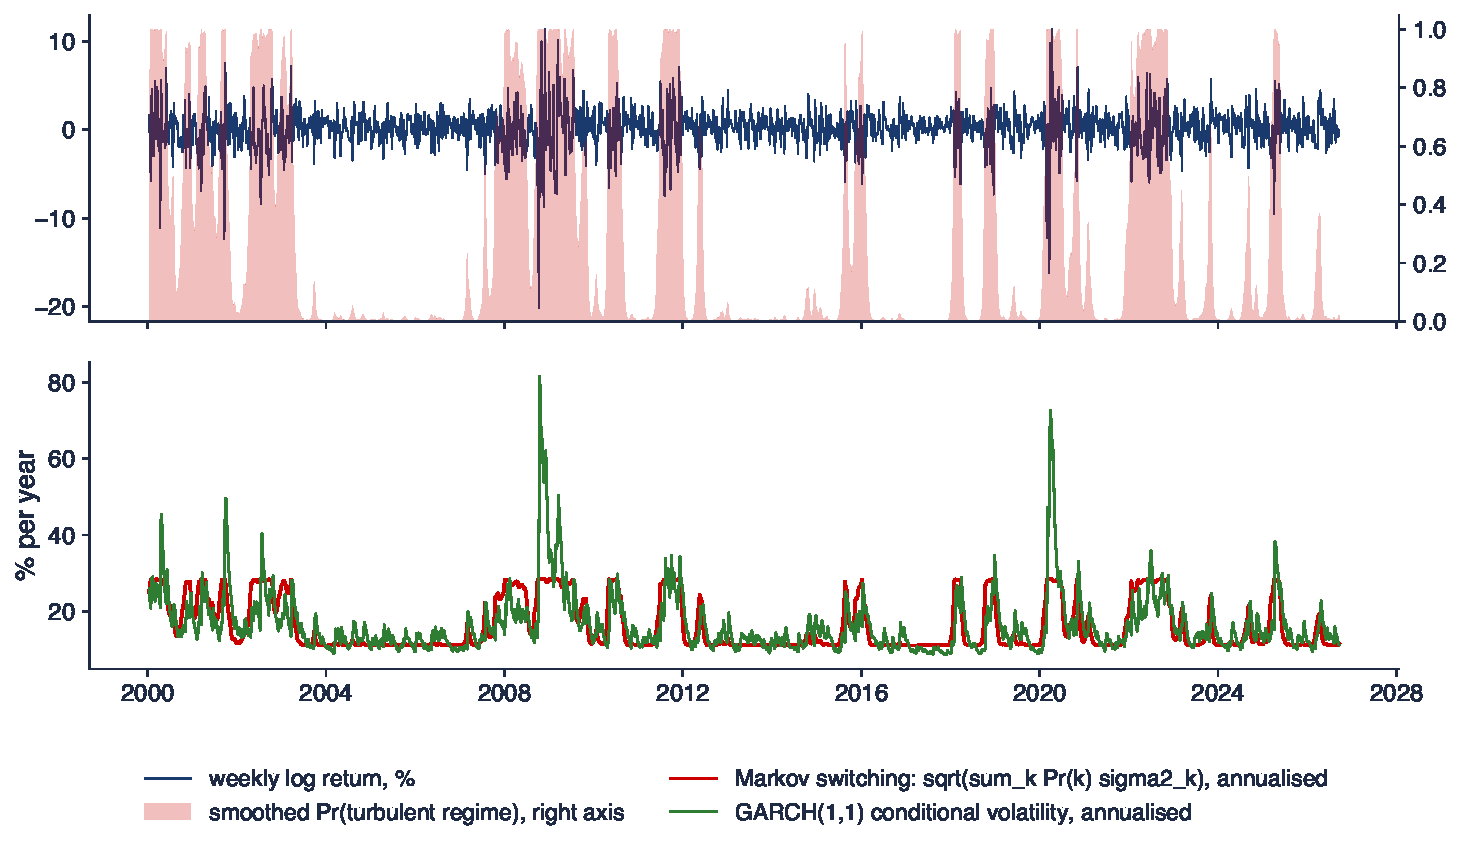
\includegraphics[width=0.97\textwidth,height=0.66\textheight,keepaspectratio]{tsa_ch10_vol_regimes.pdf}
\end{center}
\vspace{-0.25cm}
\begin{itemize}
    \item Weekly log returns of the S\&P 500, 2000--2026 (EODHD); two regimes with switching mean and variance; bottom: the volatility implied by the regime probabilities against a GARCH(1,1) (\tsachlink{https://danpele.github.io/Time-Series-Analysis/EN/Courses/chapter5_conditional_volatility_garch.pdf}{Chapter 5}), both annualised
\end{itemize}
\quantlet{TSA\_ch10\_volatility\_regimes}{\qlurl{TSA_ch10_volatility_regimes}}
\end{frame}

\begin{frame}{Interpreting the volatility regimes}
\itemsize{\small}
\begin{itemize}
    \item Calm regime: volatility 11\% per year, mean 0.32\% per week; turbulent: 28\% per year, mean \ensuremath{-}0.39\% per week
    \begin{itemize}
        \item durations: 37 weeks calm, 14 weeks turbulent; turbulent in 26\% of the weeks (ergodic 28\%)
    \end{itemize}
    \item Most turbulent years: 2022 (90\% of the weeks), 2008 (79\%), 2009 (69\%)
    \begin{itemize}
        \item correlation with the GARCH(1,1) volatility: 0.68; GARCH: $\hat\alpha = 0.26$, $\hat\beta = 0.70$
    \end{itemize}
    \item Two views of the same clustering: GARCH moves volatility continuously, the regime model jumps between two levels
\end{itemize}
\end{frame}

\begin{frame}{Regimes, GARCH persistence and long memory}
\itemsize{\small}
\begin{itemize}
    \item \refLL: shifts in the level of variance make a GARCH look almost integrated ($\alpha + \beta \approx 1$)
    \begin{itemize}
        \item the near-IGARCH estimates of \tsachlink{https://danpele.github.io/Time-Series-Analysis/EN/Courses/chapter5_conditional_volatility_garch.pdf}{Chapter 5} may reflect regimes, not one very persistent process
        \item \refHSus: ARCH within regimes (SWARCH) lowers the persistence
    \end{itemize}
    \item \refDI: rare regime switches produce a slowly decaying ACF and $\hat d > 0$ (\tsachlink{https://danpele.github.io/Time-Series-Analysis/EN/Courses/chapter8_long_memory_arfima.pdf}{Chapter 8}, spurious long memory)
    \begin{itemize}
        \item three models, one fact: volatility shocks persist; the next chart simulates the fitted regime model to see how far regimes alone go
    \end{itemize}
\end{itemize}
\end{frame}

\begin{frame}{Regimes imitate memory}
\itemsize{\footnotesize}
\begin{center}
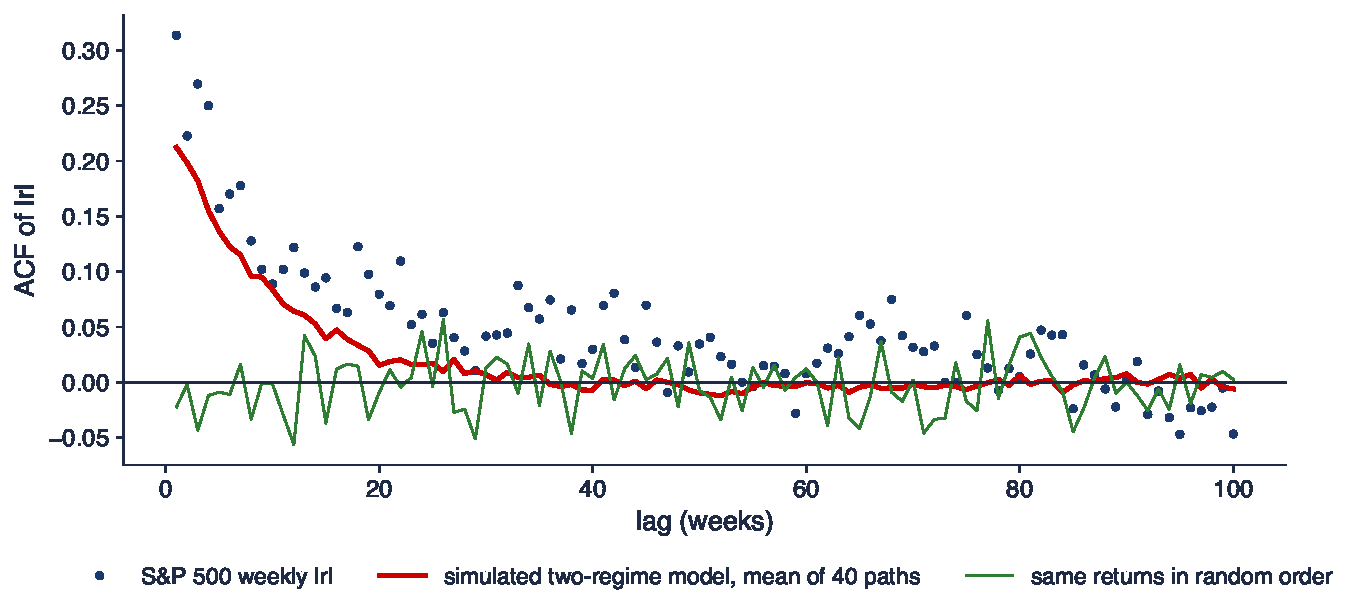
\includegraphics[width=0.97\textwidth,height=0.56\textheight,keepaspectratio]{tsa_ch10_regimes_memory.pdf}
\end{center}
\vspace{-0.25cm}
\begin{itemize}
    \item ACF of weekly $|r_t|$ of the S\&P 500; mean ACF of 40 series simulated from the fitted two-regime model (constant variance within each regime, no GARCH); the same returns in random order
\end{itemize}
\quantlet{TSA\_ch10\_volatility\_regimes}{\qlurl{TSA_ch10_volatility_regimes}}
\end{frame}

\begin{frame}{Interpreting the simulated regimes}
\itemsize{\small}
\begin{itemize}
    \item Data: ACF of $|r_t|$ 0.31 at lag 1, 0.06 at 26 weeks; regime model: 0.21 and 0.01; random order: none
    \begin{itemize}
        \item the regimes explain most of the short-run clustering, less of the long tail
    \end{itemize}
    \item Local Whittle $\hat d$ of $|r_t|$: 0.32 in the data, 0.29 (SD 0.06) in the simulated regime series, \ensuremath{-}0.05 in random order
    \begin{itemize}
        \item a GARCH(1,1) fitted to the simulated series gives $\alpha + \beta = 0.91$ on average (15 series), although there is no GARCH in them
    \end{itemize}
    \item Persistence and long memory in volatility are consistent with regimes: compare models by likelihood and forecasts, not by one statistic
\end{itemize}
\end{frame}

\begin{frame}{Recap: Markov switching}
\itemsize{\small}
\begin{itemize}
    \item $y_t = \mu_{S_t} + \varepsilon_t$, $S_t$ a Markov chain; durations $1/(1 - p_{ii})$; ergodic $\pi_1 = (1-p_{22})/(2-p_{11}-p_{22})$
    \item Hamilton filter: predict with $\mathbf{P}$, update with Bayes; Kim smoother for history
    \item US GDP: the model recovers the deep NBER recessions; filtered probabilities react later
    \item Several maxima, outliers and variance breaks can change what a ``regime'' means
    \item Regimes reproduce volatility clustering, GARCH persistence and apparent long memory
\end{itemize}
\end{frame}


%=============================================================================
\section{Possible contribution of AI}
%=============================================================================

\begin{frame}{Possible contribution of AI}
\itemsize{\small}
\begin{itemize}
    \item \textbf{Code}: a first draft of a Kalman filter, of the matrices of a new model, of a Markov-switching fit with many starting values
    \item \textbf{Explanation}: a second derivation of the gain, of the steady state, of the Hamilton filter
    \item \textbf{Exploration}: output gaps for many EU countries; regimes in many markets; a nowcast with many indicators
    \item Example prompt
    \begin{itemize}
        \item \aiprompt{Write Python code that downloads Romanian quarterly real GDP from Eurostat (namq\_10\_gdp, Q.CLV10\_MEUR.SCA.B1GQ.RO), fits UnobservedComponents with a smooth trend and an AR(2) cycle, compares the smoothed and the filtered cycle with the HP gap and with the Hamilton (2018) regression filter, and reports the revisions of the last eight quarters.}
    \end{itemize}
\end{itemize}
\end{frame}

\begin{frame}{Checks you must run}
\itemsize{\small}
\begin{itemize}
    \item Simulate from known parameters and check that the code recovers them (the Nile values of \refDK\ are a good test)
    \item Filtered or smoothed? Real-time claims need filtered estimates; an AI answer that uses \texttt{smoothed} for a ``forecast'' is wrong
    \item Durations: $1/(1 - p_{ii})$, not $p_{ii}/(1 - p_{ii})$; check the convention of the transition matrix (rows or columns) in the library
    \item Markov switching: several starting values, label switching, outliers that capture a regime
    \item The HP filter at the end of the sample: do not read the last gap as a real-time estimate
    \item Every cited reference: it must exist; check the DOI
\end{itemize}
\end{frame}


%=============================================================================
\section{Summary}
%=============================================================================

\begin{frame}{Key takeaways}
\itemsize{\small}
\begin{itemize}
    \item State space form: a hidden state $\alpha_t$ follows a VAR(1) and is measured with noise; ARMA, ETS, UC, TVP and factor models fit in it
    \item The Kalman filter predicts and updates; the gain weighs data against model; the local level filter in steady state is SES
    \item Smoothing for history, filtering for real time; the likelihood comes from the prediction errors; missing data are easy
    \item Output gaps depend on the method and are revised heavily at the end of the sample
    \item Markov switching: regime probabilities, durations $1/(1 - p_{ii})$; check what the regimes mean
\end{itemize}
\end{frame}

\begin{frame}{Key formulas}
\itemsize{\small}
{\renewcommand{\arraystretch}{1.35}\begin{center}
\footnotesize
\begin{tabular}{ll}
\toprule
\textbf{Quantity} & \textbf{Formula} \\
\midrule
State space form & $y_t = Z_t\alpha_t + \varepsilon_t$, \quad $\alpha_{t+1} = T\alpha_t + R\eta_t$ \\
Update & $v_t = y_t - Z_ta_t$, \quad $F_t = Z_tP_tZ_t' + H$, \quad $K_t = P_tZ_t'F_t^{-1}$, \quad $a_{t|t} = a_t + K_tv_t$ \\
Prediction & $a_{t+1} = Ta_{t|t}$, \quad $P_{t+1} = TP_{t|t}T' + RQR'$ \\
Local level steady state & $\bar P = \sigma^2_\varepsilon(q + \sqrt{q^2 + 4q})/2$, \quad $\alpha_{SES} = \bar K = \bar P/(\bar P + \sigma^2_\varepsilon)$ \\
Log-likelihood & $-\frac12\sum_t(\log 2\pi + \log F_t + v_t^2/F_t)$ \\
HP filter & $\min\sum(y_t - \tau_t)^2 + \lambda\sum(\Delta^2\tau_t)^2$, \quad $\lambda = \sigma^2_\varepsilon/\sigma^2_\zeta$ \\
Markov chain & $E(D_i) = 1/(1 - p_{ii})$, \quad $\pi_1 = (1 - p_{22})/(2 - p_{11} - p_{22})$ \\
Hamilton filter & $\Pr(S_t = j \mid Y_t) \propto f_j(y_t)\sum_i p_{ij}\Pr(S_{t-1} = i \mid Y_{t-1})$ \\
\bottomrule
\end{tabular}
\end{center}
}
\end{frame}

\begin{frame}{Self-assessment}
\itemsize{\small}
\begin{itemize}
    \item \textbf{Question}: local level with $P_t = 3$, $\sigma^2_\varepsilon = 1$. What is the Kalman gain?
    \begin{itemize}
        \item \textbf{Answer}: $K_t = 3/(3 + 1) = 0.75$: the new observation gets weight 0.75
    \end{itemize}
    \item \textbf{Question}: an SES model has $\alpha = 0.5$. Which local level model is behind it?
    \begin{itemize}
        \item \textbf{Answer}: $q = \alpha^2/(1 - \alpha) = 0.25/0.5 = 0.5$
    \end{itemize}
    \item \textbf{Question}: $p_{11} = 0.9$ in a two-regime model. How long does regime 1 last on average?
    \begin{itemize}
        \item \textbf{Answer}: $1/(1 - 0.9) = 10$ periods
    \end{itemize}
    \item Next: \tsachlink{https://danpele.github.io/Time-Series-Analysis/EN/Courses/chapter11_foundation_models_time_series.pdf}{Chapters 11}--\tsachlink{https://danpele.github.io/Time-Series-Analysis/EN/Courses/chapter14_multivariate_garch_models.pdf}{14} for self-study; \tsachlink{https://danpele.github.io/Time-Series-Analysis/EN/Courses/chapter15_review.pdf}{Chapter 15}, review
\end{itemize}
\end{frame}


%=============================================================================
\section{References}
%=============================================================================

\begin{frame}{References (1/2)}
\itemsize{\tiny}
\begin{itemize}
    \item Chauvet, M., \& Piger, J. (2008). A comparison of the real-time performance of business cycle dating methods. \textit{Journal of Business \& Economic Statistics}, 26(1), 42--49. \href{https://doi.org/10.1198/073500107000000296}{doi:10.1198/073500107000000296}
    \item Diebold, F. X., \& Inoue, A. (2001). Long memory and regime switching. \textit{Journal of Econometrics}, 105(1), 131--159. \href{https://doi.org/10.1016/S0304-4076(01)00073-2}{doi:10.1016/S0304-4076(01)00073-2}
    \item Durbin, J., \& Koopman, S. J. (2012). \textit{Time Series Analysis by State Space Methods} (2nd ed.). Oxford University Press. \href{https://doi.org/10.1093/acprof:oso/9780199641178.001.0001}{doi:10.1093/acprof:oso/9780199641178.001.0001}
    \item Giannone, D., Reichlin, L., \& Small, D. (2008). Nowcasting: The real-time informational content of macroeconomic data. \textit{Journal of Monetary Economics}, 55(4), 665--676. \href{https://doi.org/10.1016/j.jmoneco.2008.05.010}{doi:10.1016/j.jmoneco.2008.05.010}
    \item Hamilton, J. D. (1989). A new approach to the economic analysis of nonstationary time series and the business cycle. \textit{Econometrica}, 57(2), 357--384. \href{https://doi.org/10.2307/1912559}{doi:10.2307/1912559}
    \item Hamilton, J. D. (1990). Analysis of time series subject to changes in regime. \textit{Journal of Econometrics}, 45(1--2), 39--70. \href{https://doi.org/10.1016/0304-4076(90)90093-9}{doi:10.1016/0304-4076(90)90093-9}
    \item Hamilton, J. D. (1994). \textit{Time Series Analysis}. Princeton University Press. \href{https://doi.org/10.2307/j.ctv14jx6sm}{doi:10.2307/j.ctv14jx6sm}
    \item Hamilton, J. D. (2018). Why you should never use the Hodrick--Prescott filter. \textit{The Review of Economics and Statistics}, 100(5), 831--843. \href{https://doi.org/10.1162/rest\_a\_00706}{doi:10.1162/rest\_a\_00706}
    \item Hamilton, J. D., \& Susmel, R. (1994). Autoregressive conditional heteroskedasticity and changes in regime. \textit{Journal of Econometrics}, 64(1--2), 307--333. \href{https://doi.org/10.1016/0304-4076(94)90067-1}{doi:10.1016/0304-4076(94)90067-1}
    \item Harvey, A. C. (1989). \textit{Forecasting, Structural Time Series Models and the Kalman Filter}. Cambridge University Press. \href{https://doi.org/10.1017/CBO9781107049994}{doi:10.1017/CBO9781107049994}
    \item Harvey, A. C., \& Jaeger, A. (1993). Detrending, stylized facts and the business cycle. \textit{Journal of Applied Econometrics}, 8(3), 231--247. \href{https://doi.org/10.1002/jae.3950080302}{doi:10.1002/jae.3950080302}
    \item Hodrick, R. J., \& Prescott, E. C. (1997). Postwar U.S. business cycles: An empirical investigation. \textit{Journal of Money, Credit and Banking}, 29(1), 1--16. \href{https://doi.org/10.2307/2953682}{doi:10.2307/2953682}
    \item Huang, C., \& Petukhina, A. (2022). \textit{Applied Time Series Analysis and Forecasting with Python}. Springer. \href{https://doi.org/10.1007/978-3-031-13584-2}{doi:10.1007/978-3-031-13584-2}
    \item Hyndman, R. J., Koehler, A. B., Ord, J. K., \& Snyder, R. D. (2008). \textit{Forecasting with Exponential Smoothing: The State Space Approach}. Springer. \href{https://doi.org/10.1007/978-3-540-71918-2}{doi:10.1007/978-3-540-71918-2}
    \item Kalman, R. E. (1960). A new approach to linear filtering and prediction problems. \textit{Journal of Basic Engineering}, 82(1), 35--45. \href{https://doi.org/10.1115/1.3662552}{doi:10.1115/1.3662552}
    \item Kim, C.-J. (1994). Dynamic linear models with Markov-switching. \textit{Journal of Econometrics}, 60(1--2), 1--22. \href{https://doi.org/10.1016/0304-4076(94)90036-1}{doi:10.1016/0304-4076(94)90036-1}
\end{itemize}
\end{frame}

\begin{frame}{References (2/2)}
\itemsize{\tiny}
\begin{itemize}
    \item Kim, C.-J., \& Nelson, C. R. (1999). \textit{State-Space Models with Regime Switching: Classical and Gibbs-Sampling Approaches with Applications}. MIT Press. \href{https://doi.org/10.7551/mitpress/6444.001.0001}{doi:10.7551/mitpress/6444.001.0001}
    \item Lamoureux, C. G., \& Lastrapes, W. D. (1990). Persistence in variance, structural change, and the GARCH model. \textit{Journal of Business \& Economic Statistics}, 8(2), 225--234. \href{https://doi.org/10.1080/07350015.1990.10509794}{doi:10.1080/07350015.1990.10509794}
    \item Muth, J. F. (1960). Optimal properties of exponentially weighted forecasts. \textit{Journal of the American Statistical Association}, 55(290), 299--306. \href{https://doi.org/10.1080/01621459.1960.10482064}{doi:10.1080/01621459.1960.10482064}
    \item Rauch, H. E., Tung, F., \& Striebel, C. T. (1965). Maximum likelihood estimates of linear dynamic systems. \textit{AIAA Journal}, 3(8), 1445--1450. \href{https://doi.org/10.2514/3.3166}{doi:10.2514/3.3166}
    \item Shumway, R. H., \& Stoffer, D. S. (2017). \textit{Time Series Analysis and Its Applications} (4th ed.). Springer. \href{https://doi.org/10.1007/978-3-319-52452-8}{doi:10.1007/978-3-319-52452-8}
    \item Stock, J. H., \& Watson, M. W. (1989). New indexes of coincident and leading economic indicators. \textit{NBER Macroeconomics Annual}, 4, 351--394. \href{https://doi.org/10.1086/654119}{doi:10.1086/654119}
\end{itemize}
\end{frame}

\end{document}
